\documentclass[12pt]{article}
% Packages
\usepackage[utf8]{inputenc}
\usepackage[T1]{fontenc}
\usepackage{lipsum} % For dummy text
\usepackage{physics} % For physics notation
\usepackage{amsmath} % For math
\usepackage{amssymb} % For math symbols 
\usepackage[margin=2cm]{geometry} % For smaller margins
\usepackage{gensymb} % For degree symbol
\usepackage{diagbox} % For table
\usepackage{slashbox} % For table
% \usepackage[margin=1in,headheight=57pt,headsep=0.1in]{geometry}
\usepackage{hyperref}
\usepackage{xcolor} % for colored text
\usepackage{graphicx} % For \includegraphics
\usepackage{float}    % For the [H] placement specifier
% \usepackage{biblatex} %Imports biblatex package
\usepackage[
backend=biber,
style=alphabetic,
sorting=ynt
]{biblatex}
\addbibresource{bib.bib} %Import the bibliography file

% Document information
\title{FYP Report}
\author{Lin Zhonglin}
\date{\today}
\usepackage{setspace}
% Using \doublespacing in the preamble 
% changes the text to double-line spacing
\doublespacing
\begin{document}
\noindent

\maketitle
\tableofcontents

\section{Overview}
%%%%%% 草稿 %%%%%%%%
% \begin{enumerate}
%     \item Background: 
%     \item Key part of my work: (depends on how far I go)
%         \begin{enumerate}
%             \item The optimised pulse for a particular state preparation
%             \item how it differs from other pulse (Chiyuan's alternate pulse way)
%             \item Go from model Hamiltonian to physical Hamiltonain, 
%                     discuss the approximations' effect, 
%                     compare fideilty
%         \end{enumerate}
% \end{enumerate}

% TODO: 
% \begin{enumerate}
%     \item Go through the Hamiltonian derivation 
%             $\rightarrow$ for comparison of fidelity later 
%     \item does Qutip considers the cavity Hilbert space truncation discussed below? 
% \end{enumerate}


% Issues to be dealt with: 
% \begin{enumerate}
%     \item local minima / maxima in optimization algorithm
%     \item Reinhold: 
%         Optimizing a full unitary operation is sensible for qubits, or systems of a few qubits, but in the cavity manipulations to be performed in the following sections, this is not usually a sensible operation, since doing operations involving states at the border of the truncation (i.e. the maximum photon number state considered in the simulation), would typically require a larger truncation to simulate accurately (driving $\ket{n_{ph}}$) will almost always in part bring us partially to $\ket{n_{ph} + 1}$.
% \end{enumerate}
%%%%%% 草稿 %%%%%%%%
% quantum computing -> continuous quantum computing -> transmon-cavity -> DQD-cavity -> state preparation -> pulse optimization -> 
Quantum computing leverages quantum mechanics principles, using qubits that can exist in multiple states simultaneously, enabling parallel processing. 
Various physical implementations such as superconducting qubits, trapped ions, and quantum dots have emerged as possible quantum computing platforms.
Besides traditional discrete quantum variable quantum computing where qubits represent binary states, an emerging continuous variable quantum computing uses multiple physical qubits to encode logical qubits, offering a different approach to error correction. \cite{RevModPhys.77.513}
One common platform for continuous variable quantum computing is cavity coupled to an auxiliary qubit for control.
This is often termed "bosonic qubits in circuit QED".\cite{Joshi_2021} In this area of quantum computing, the common physical platform is cavity coupled to a transmon. In this report we consider a possible alternative, cavity coupled to a Double Quantum Dot (DQD). \cite{D_Anjou_2019}
State preparation is crucial, as it initializes qubits for computation, with accuracy impacting the overall performance of quantum algorithms. \cite{Nielsen2010}
In this report I focus on control pulse optimization for state preparation of a cavity cat state on a cavity-DQD physical system. 
Pulse optimization was successfully run for effective Hamiltonian (in restricted regime) of the system to arbitrarily high fidelity. (higher fidelity, longer computation time)
However, the fidelity of the optimized pulses when run using the full physical Hamiltonian couldn't be attained in reasonable computation time. 
Details can be seen in section \ref{sec:future_work}.




%%%%%%%%%%%%%%%%%%%%%%%%%%%%%%%%%%%%%%%%%%%%%%%%%%%%%%%%%%%%%%%
\section{Background, theory and motivation}
%%%%%% 草稿 %%%%%%%%
% content: 
% introduce the idea of bosonic-modes-encoded qubits, give a simple example;
%  motivate Bosonic-modes-encoded qubits 
%     -> that one physical device now can encode multiple qubits
%     -> this also makes error correction more efficient -> easier to control multiple qubits

% introduce cavity-transmon system 
% motivate for cavity-DQD system

% theory of cavity-DQD: 
% original Hamiltonians -> rotation, approximaition, dispersive regime, etc... -> the Hamiltonian I used for pulse optimization


%%%%%% 草稿 %%%%%%%%
%%%%%%%%%%%%%%%%%%%%%%%%%%%%%%%
\subsection{bosonic-modes-encoded qubits}
Quantum computing has emerged as a paradigm with the potential to solve problems that are intractable for classical computers. Among the various physical implementations of qubits, the cavity-coupled transmon system has become a leading platform due to its strong nonlinearity and large Hilbert space. This system leverages the coupling between the transmon qubit and the cavity to achieve robust qubit control and readout \cite{blais2004, houck2008}.

One of the key advantages of using a cavity for quantum computing is its potential for quantum error correction. By encoding a single logical qubit into multiple cavity Fock states, it is possible to protect against certain types of errors, thus enhancing the reliability of quantum computations \cite{girvin2014, ofek2016}.

Despite the success of the cavity-coupled transmon system, there is ongoing research into alternative qubit implementations that may offer further advantages. One such alternative is the cavity-coupled Double Quantum Dot (DQD) system. This system combines the advantages of semiconductor quantum dots, such as scalability and compatibility with existing semiconductor technology, with the strong coupling and large Hilbert space provided by the cavity. The DQD system has the potential to achieve high-fidelity qubit operations while maintaining the error correction capabilities of cavity-based systems \cite{Mi2018}.

The control and manipulation of quantum systems are central to the realization of quantum computing. Quantum optimal control theory provides a framework for designing control protocols that achieve desired quantum operations with high fidelity. In this context, the goal is to find optimal control fields that drive the evolution of the quantum system from an initial state to a target state or implement a specific unitary transformation. Techniques such as Gradient Ascent Pulse Engineering (GRAPE) and Chopped Random Basis (CRAB) optimization are commonly used to find these optimal control fields \cite{KHANEJA2005296}. These methods involve numerically optimizing a cost function, typically related to the fidelity between the achieved and desired quantum states, subject to constraints imposed by the physical system and control hardware.

In this report, we explore the application of quantum optimal control theory to the cavity-coupled DQD system for state preparation tasks. We compare the performance of different control optimization algorithms and investigate the effects of various approximations and constraints on the control fidelity. Through this study, we aim to demonstrate the potential of the cavity-coupled DQD system as a platform for quantum computing and contribute to the development of robust control techniques for quantum technologies.

% gpt

Quantum computing is a revolutionary technology that leverages the principles of quantum mechanics to perform calculations at speeds unattainable by classical computers. Unlike classical computers, which use bits as the basic unit of information (either 0 or 1), quantum computers use quantum bits, or qubits, which can exist in a superposition of both 0 and 1 simultaneously. This property, along with entanglement and interference, enables quantum computers to process a vast amount of information in parallel, making them potentially capable of solving certain complex problems much more efficiently than classical computers \cite{Nielsen2010}.

There are several physical implementations of quantum computers, each with its unique advantages and challenges. Some of the most prominent include:

Superconducting Qubits: These are the most widely used and are based on superconducting circuits cooled to extremely low temperatures. Companies like IBM and Google use this approach in their quantum computers \cite{devoret2013superconducting}.
Trapped Ions: In this implementation, ions are trapped using electromagnetic fields and manipulated with lasers. It offers high precision and long coherence times but can be challenging to scale up \cite{blatt2012quantum}.
Topological Qubits: Based on exotic particles called anyons, topological qubits are believed to be more resistant to errors, but the technology is still in its early stages \cite{kitaev2003fault}.
Quantum Dots and Silicon-based Qubits: These approaches aim to leverage semiconductor manufacturing techniques to build scalable quantum computers \cite{loss1998quantum}.
In traditional quantum computing, qubits are encoded using two-level systems, where each qubit can represent a 0 or a 1 in a superposition. In contrast, continuous variable quantum computing uses continuous degrees of freedom, such as the position and momentum of a particle, to represent quantum information. This allows for the encoding of logical qubits onto multiple physical qubits, offering a different approach to error correction and information processing \cite{weedbrook2012gaussian}.

State preparation is a crucial step in quantum computing, as it involves initializing the qubits in a specific quantum state before any computation can begin. The accuracy of state preparation directly impacts the reliability and performance of quantum algorithms. Errors in state preparation can propagate throughout the computation, leading to incorrect results. Additionally, many quantum algorithms, such as those for quantum simulation or quantum machine learning, require the preparation of complex quantum states as their initial step. Therefore, developing techniques for precise and efficient state preparation is essential for the advancement of quantum computing \cite{nielsen2002quantum}.

In summary, quantum computing is a cutting-edge field that exploits the principles of quantum mechanics to achieve computational power beyond the reach of classical computers. Its development involves various physical implementations, each with its own set of challenges and advantages. The distinction between traditional qubits and continuous variable quantum computing offers different avenues for error correction and information processing. Finally, state preparation is a critical aspect of quantum computing, as it sets the stage for accurate and effective quantum computations.

%%%%%%%%%%%%%%%%%%%%%%%%%%%%%%%
\subsection{Physical systems and Hamiltonians}
%%%%%% 草稿 %%%%%%%%
% discuss 
% - Full Original Hamiltonian 
% - effective Hamiltonian (same as )
% main papers: 
% - Optimal dispersive readout of a spin qubit with a microwave resonator

% why is cavity coupled to QDQ spin intresting
% DQD Hamiltonian
%%%%%% 草稿 %%%%%%%%
Strong coupling of semiconductor spin qubits to superconducting microwave resonators was recently demonstrated. \cite{Mi2018}\cite{Landig2018}
These breakthroughs can potentially combine the long coherence times of solid-state spin qubits with the long-distance connectivity, fast control, and fast high-fidelity quantum-non-demolition readout of existing superconducting qubit implementations.\cite{D_Anjou_2019}
We consider a DQD defined by a double-well potential $V(z)$ whose wells are separated by a distance $2d$, as depicted in Fig \ref{fig:DQD}.
The two lowest-energy orbitals of the right and left wells are labelled $|\widetilde{R}\rangle$ and $|\widetilde{L}\rangle$, respectively, with corresponding energies $\epsilon_R$ and $\epsilon_L$.
The energy detuning between the right and left orbitals is $\epsilon=\epsilon_R-\epsilon_L$, and the tunnel coupling between them is $t_c>0$. 
Moreover, a uniform longitudinal magnetic field is applied along the axis of the quantum dot (the $z$ axis). This induces a Zeeman energy splitting $\hbar \gamma_e B_z$ of the electronic spin states $|\widetilde{\uparrow}\rangle$ and $|\widetilde{\downarrow}\rangle$, where $\gamma_e$ is the electron gyromagnetic ratio. 
In addition, a transverse position-dependent magnetic field $B_x(z)$ is applied along the $x$ axis using, e.g., a proximal micromagnet. As the electron moves across the DQD, it therefore experiences a magnetic field variation of order $b_x=\partial_z B_x(z) \times d$. This hybridizes the spin and charge degrees of freedom, enabling electrical control and readout of the spin. 
In the following, we set $\hbar=1$ and $\gamma_e=1$. The resulting DQD Hamiltonian is
\begin{equation}\label{eq:DQD_Hamiltonian}
    \begin{aligned} 
        & H_d=H_m+H_Z, \\
        & H_m=\frac{\epsilon}{2} \widetilde{\tau}_z+t_c \widetilde{\tau}_x, \\
        & H_Z=\frac{B_z}{2} \widetilde{\sigma}_z+\frac{b_x}{2} \widetilde{\tau}_z \widetilde{\sigma}_x .
    \end{aligned}    
\end{equation}


In Eq. \ref{eq:DQD_Hamiltonian}, $H_m$ is the molecular Hamiltonian of the DQD and $H_Z$ is the Zeeman Hamiltonian. Moreover, the $\widetilde{\tau}_i$ are the Pauli matrices in the $\{|\widetilde{R}\rangle,|\widetilde{L}\rangle\}$ basis and the $\widetilde{\sigma}_i$ are the Pauli matrices in the $\{|\widetilde{\uparrow}\rangle,|\widetilde{\downarrow}\rangle\}$ basis. 
It is also convenient to introduce the eigenstates $|\widetilde{ \pm}\rangle$ of the molecular Hamiltonian $H_m$. They satisfy $H_m|\widetilde{\Psi}\rangle= \pm \frac{\Omega}{2}|\widetilde{\Psi}\rangle$, where $\Omega=\sqrt{\left(2 t_c\right)^2+\epsilon^2}=2 t_c \sec \theta$ is the molecular energy gap and where $\theta=\arctan \left(\epsilon / 2 t_c\right)$ is the molecular mixing angle. 
Note that the description of electronic motion in terms of the two lowest-energy orbitals is only valid in the limit where $\Omega$ is much smaller than the single-dot orbital splitting, whether it originates from confinement or from valley splitting.
\begin{figure}[H]
    \centering
    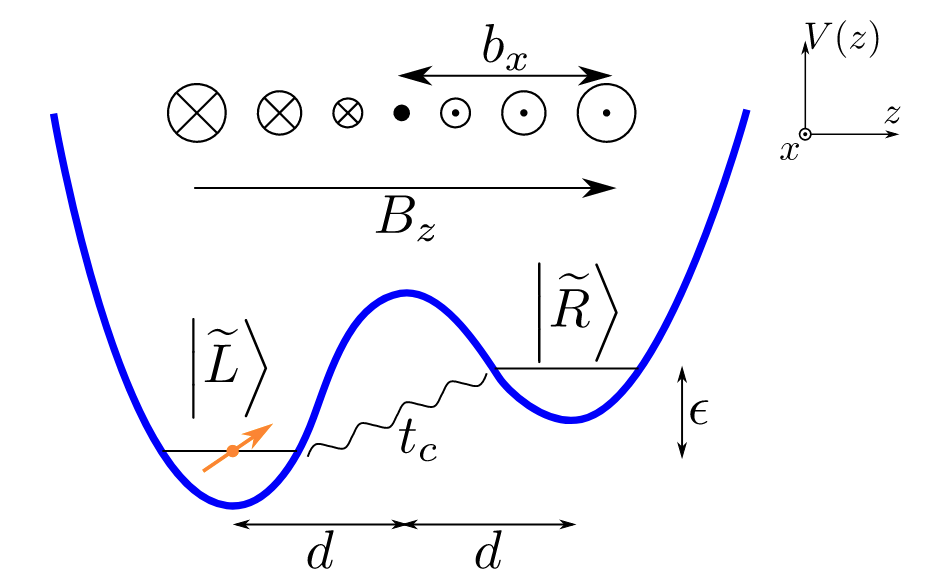
\includegraphics[width=0.5\linewidth]{DQD.png}
    \caption{
        (a) Schematic representation of the double-well potential $V(z)$ forming the DQD. The detuning and tunnel coupling between the right dot orbital $|\widetilde{R}\rangle$ and left dot orbital $|\widetilde{L}\rangle$ are $\epsilon$ and $t_c$, respectively. The DQD is subject to a longitudinal magnetic field $B_z \hat{z}$ and an external transverse magnetic field gradient $\partial_z B_x(z) \hat{x}$ such that the field $B_x$ varies by $b_x=\partial_z B_x(z) \times d$ over the half interdot distance $d$. (b) Setup for the dispersive readout of a DQD embedded in a two-port microwave resonator with resonance frequency $\omega_r$. The DQD and the resonator electric field (green arrows) interact via the electric dipole coupling $g_c$. The resonator can be driven in the $i$ th port by an input field $b_i^{\text {in }}(t)$. The output fields $b_i^{\text {out }}(t)$ then carry information on the state of the DQD. The leakage rates of ports 1 and 2 to their respective feedlines are $\kappa_1$ and $\kappa_2$.
    }
    \label{fig:DQD}
\end{figure}

% Double-quantum-dot-resonator interaction
The electric field of the resonator couples directly to the electric dipole moment of the electron, as shown schematically in Fig. \ref{fig:DQD}(b). 
Due to the interaction of the spin and orbit degrees of freedom in Eq. \ref{eq:DQD}, the resonator photons can drive spin transitions. 
The Hamiltonian of the combined resonator and DQD system is
\begin{equation}\label{eq:DQD_resonator_Hamiltonian}
    \begin{aligned} 
        & H=H_d+H_r+V, \\
        & H_r=\omega_r a^{\dagger} a, \\    
    & V=g_c \tilde{\tau}_z\left(a+a^{\dagger}\right) .
    \end{aligned}
\end{equation}

In Eq. \ref{eq:DQD_resonator_Hamiltonian}, $H_r$ is the free Hamiltonian for a single mode of the resonator, $V$ is the dipole interaction Hamiltonian between the electron and the resonator, and $a$ annihilates a photon in the resonator. 
The resonance frequency of the resonator is $\omega_r>0$ and the strength of the dipole coupling is $g_c$.

% Double-quantum-dot eigenbasis and spin qubit
The DQD Hamiltonian, Eq. (1), can be diagonalized exactly as detailed in Appendix A. Expressed in its eigenbasis, the Hamiltonian $H_d$ takes the form
\begin{equation}\label{eq:DQD_Hamiltonian_in_eigenbasis}
    H_d=\frac{E_m}{2} \tau_z+\frac{E_s}{2} \sigma_z,    
\end{equation}

where the $\tau_i$ and the $\sigma_i$ are now Pauli matrices in the eigenbasis $\left|\tau_z ; \sigma_z\right\rangle$ of $H_d$ dressed by the field gradient. 
Here $\tau_z= \pm$ labels the dressed "molecular-like" states and $\sigma_z=\uparrow(\downarrow)$ labels the dressed "spin-like" states [67]. 
Exact expressions for the molecular-like and spin-like Larmour frequencies $E_m$ and $E_s$ are derived in Appendix A. The energy-level diagram of the DQD is illustrated in Fig. 2, where we have also introduced the transition frequencies $E_{ \pm}=E_m \pm E_s$. 
In the following, we consider the spin qubit formed from the two dressed spin-like eigenstates spanning the molecular ground state. 
Specifically, we choose the computational basis $\{|1\rangle,|0\rangle\}=$ $\{|-; \uparrow\rangle,|-; \downarrow\rangle\}$. 
Despite their spin-like character, the electric dipole matrix element between these two states is finite and transitions between them can be induced electrically. 
In particular, the DQD-resonator interaction of Eq. (2) is written in the new basis as
\begin{equation}\label{eq:DQD_resonator_interaction_new_basis}
    \begin{aligned}
        V= & \mathcal{V}\left(a+a^{\dagger}\right), \\
        \mathcal{V}= & -g_m \tau_x+g_s \tau_z \sigma_x+g_{+}\left(\tau_{+} \sigma_{+}+\tau_{-} \sigma_{-}\right) \\
        & +g_{-}\left(\tau_{+} \sigma_{-}+\tau_{-} \sigma_{+}\right)+g_{m p} \tau_z+g_{s p} \sigma_z .
        \end{aligned}    
\end{equation}

Here $\left\{g_m, g_s, g_{+}, g_{-}\right\}$are the coupling strengths of the resonator to the DQD transitions of frequencies $\left\{E_m, E_s, E_{+}, E_{-}\right\}$ illustrated in Fig. 2. 
In addition, $g_{m p}$ and $g_{s p}$ are couplings arising from the finite dc electric polarizabilities of the molecular electric dipole and of the spin, respectively. 
Exact expressions for the $g_i$ are given in Appendix A. In Eq. (10), the term $g_s \tau_z \sigma_x\left(a+a^{\dagger}\right)$ exchanges energy between the resonator and the spin qubit. It can thus be exploited for resonatorassisted qubit control and readout. 
As will be discussed in Sec. IV F, the couplings $g_{ \pm}$of the resonator to the transitions of frequencies $E_{ \pm}$can also be harnessed to improve readout performance.

In the remainder of this article, we focus on the limit of weak field gradient. In particular, we assume that the direction of the spin quantization axis is not substantially modified by the presence of the field gradient, $\left|b_x \sin \theta\right| \ll$ $\left|B_z\right|$. Moreover, we assume that the admixture of spin and orbit is weak, $\left|b_x \cos \theta\right| \ll \min \left(\left|\Omega-B_z\right|,\left|\Omega+B_z\right|\right)$. Under these conditions, the dressed molecular and spin Larmour frequencies are
\begin{equation}\label{eq:Larmour_frequencies}
    \begin{aligned}
        & E_m \approx \Omega+\frac{b_x}{2} \cos \theta \sin \bar{\phi}, \\
        & E_s \approx B_z-\frac{B_z}{2} \frac{b_x}{2 t_c}\left(1-\frac{\epsilon^2}{B_z^2}\right) \sin \bar{\phi}, \\
        & \sin \bar{\phi} \approx \frac{2 t_c b_x}{\Omega^2-B_z^2},
    \end{aligned}
\end{equation}
where $\bar{\phi} \ll \pi / 2$ is the effective spin-orbit mixing angle arising from the field gradient. Approximate expressions may also be obtained for the couplings $g_i$. In particular, the molecularphoton coupling $g_m$ and spin-photon coupling $g_s$ become
\begin{equation}\label{eq:couplings}
    g_m \approx g_c \cos \theta \cos \bar{\phi}, \quad g_s \approx g_c \cos \theta \sin \bar{\phi} .
\end{equation}

% Dispersive Hamiltonian
%  Dispersive limit
Dispersive readout of the spin is performed by probing the resonator near its resonance frequency, $\omega_{\text {in }} \approx \omega_r$, and observing the spin-dependent phase of the output field. For many quantum information processing tasks, it is highly desirable that the readout perturbs the system as little as possible. To minimize such unwanted backaction on the system, we work in the so-called dispersive limit. In that limit, all DQD-resonator interaction terms in Eq. (10) are off-resonant. A given interaction term is off-resonant if its magnitude is smaller than the detuning of the resonator with the transition it induces. Let $\langle n\rangle \approx 4 \kappa_i\left|\beta_i^{\text {in }}\right|^2 / \kappa^2$ be the average number of photons entering the resonator from port $i$. Noting that the resonator field is of order $a \sim \sqrt{\langle n\rangle}$, it is easily verified that a term $\propto g_j$ in Eq. (10) is off-resonant if $\langle n\rangle$ is smaller than the so-called critical photon number,
$$
n_{c, j} \approx \frac{1}{4} \max \left(\left|\eta_j\right|,\left|\eta_j^{\prime}\right|\right)^{-2} .
$$

Here $\left|\eta_j\right| \ll 1$ and $\left|\eta_j^{\prime}\right| \ll 1$ are the small dimensionless parameters that control the dispersive limit. They have the form (see Appendix B for details)
$$
\eta_j=\frac{2 E_j g_j}{\omega_r^2-E_j^2}, \quad \eta_j^{\prime}=\frac{\omega_r}{E_j} \eta_j .
$$

The condition $\langle n\rangle<n_{c, j}$ ensures that the probe photons excite a given transition between eigenstates of $H$ at a rate that is smaller than the relaxation rate for that transition [68]. Thus, the condition $\langle n\rangle<n_{c, j}$ ensures that probe photons close to resonance with a given transition $j$ excite that transition with negligible probability [69]. A detailed analysis of these transition rates and their effect on readout is beyond the scope of this work. In the following, we will reserve the symbol $n_c$ for the critical photon number of the spin transition, $n_c \equiv n_{c, s}$.

In the dispersive limit, the Hamiltonian, Eq. (2), can be diagonalized to first order in $g_c$ using a Schrieffer-Wolff
transformation. The resulting dispersive Hamiltonian for the DQD-resonator interaction is derived in Appendix B and has the form
$$
H_{\text {dis }}=H_0+V_{\text {dis }}+V_{\text {tr }} .
$$

Here $H_0=H_d+H_r$ is the free Hamiltonian. The interaction is separated into a dispersive part $V_{\text {dis }}$ that commutes with $H_0$ and a transition-inducing part $V_{\mathrm{tr}}$ that does not commute with $H_0$. The dispersive interaction has the form:
$$
V_{\mathrm{dis}}=-\frac{1}{2} \chi_0 \tau_z \sigma_z-\left(\chi_m \tau_z+\chi_s \sigma_z\right)\left(a^{\dagger} a+\frac{1}{2}\right) .
$$

Here $\chi_m \tau_z$ and $\chi_s \sigma_z$ are the dispersive energy shifts of the resonator frequency due to coupling with the molecular electric dipole and the spin, respectively. In addition, $-\chi_0 \tau_z \sigma_z / 2$ is an Ising-like dispersive interaction between the molecular electric dipole and the spin. Expressions for $\chi_m, \chi_s$, and $\chi_0$ are given in Appendix B. As discussed in Sec. III B, the spin dispersive shift, $\chi_s \sigma_z$, may be exploited for dispersive readout of the spin. Contrary to the dispersive interaction, the offdiagonal term $V_{\text {tr }}$ induces transitions between the eigenstates of $H_0$. Specifically, $V_{\mathrm{tr}}$ can generate all the DQD transitions of Fig. 2 via the exchange of either 0 or 2 photons with the resonator. Thus, a transition term inducing a transition $j$ can be neglected if its magnitude is smaller than $\omega_r,\left|E_j\right|$, and $\left|2 \omega_r \pm E_j\right|$ (a concrete example is given in Appendix C). These off-resonance conditions can be seen as a higher-order dispersive approximation. They ensure that the operators appearing in Eq. (16) are expressed in a basis that is close to the true eigenbasis of the full system Hamiltonian $H$. If the transition term becomes resonant, the resulting change of basis enables probe photons to generate new transitions between the system eigenstates. The above off-resonance conditions are typically satisfied in the dispersive limit (though not always, see Fig. 5). We will therefore ignore the transition term in the following analysis until stated otherwise.

% Effective spin-qubit Hamiltonian
In the absence of photon-induced DQD transitions, the dispersive Hamiltonian, Eq. (16), may safely be projected into the logical subspace of the spin qubit to obtain an effective dispersive Hamiltonian for the spin qubit, in the form (up to an irrelevant constant):
$$
H_{\mathrm{dis}}^{\mathrm{eff}}=\left(\omega_r^{\prime}-\chi_s \sigma_z\right) a^{\dagger} a+\frac{1}{2}\left(E_s^{\prime}-\chi_s\right) \sigma_z .
$$

Here $\omega_r^{\prime}=\omega_r+\chi_m$ and $E_s^{\prime}=E_s+\chi_0$ are renormalized resonator and spin-qubit frequencies, respectively. In addition, $\chi_s \sigma_z$ is the spin-state-dependent dispersive shift of the resonator frequency which enables dispersive readout. The full expression for the dispersive shift is
$$
\chi_s=\frac{2 E_s g_s^2}{\omega_r^2-E_s^2}+\frac{E_{+} g_{+}^2}{\omega_r^2-E_{+}^2}-\frac{E_{-} g_{-}^2}{\omega_r^2-E_{-}^2} .
$$

When the resonator is close to resonance with the spin transition but far detuned from $E_{+}$and $E_{-}$, the dispersive shift takes the more familiar form $\chi_s \approx g_s^2 / \Delta$, where $\Delta=\omega_r-E_s$ is the spin-resonator detuning. We will assume that this is the case for most of the analysis of Sec. IV. In Sec. IV F, however, we will see that the various contributions in Eq. (18) can interfere constructively and thereby significantly improve

readout performance. This mirrors the so-called straddling regime of superconducting qubits [57-60]. Finally, note that the renormalization of the resonator and spin frequencies are unimportant for the optimization of the dispersive readout. As discussed in Sec. IV B, the readout response only depends on the detuning between the probe frequency $\omega_{\text {in }}$ and the renormalized resonator frequency $\omega_r^{\prime}$. Thus, the renormalization of the $\omega_r$ can always be compensated by adjusting $\omega_{\text {in }}$. Moreover, inspection of the expression for $\chi_0$ given in Appendix B shows that $\chi_0 \lesssim \chi_s \ll \Delta$ near the DQD-resonator resonances. Therefore, the renormalization of the spin frequency may safely be neglected.

All operators appearing in Eq. (17), and in particular $\sigma_z$, are dressed by the DQD-resonator interaction to first order in $g_c$. Thus, the spin qubit we consider is in fact formed by the states $\{|-; \uparrow\rangle,|-; \downarrow\rangle\}$ dressed by resonator photons. In the regime where both the resonator and the qubit are near-resonant with the probe, the effective driving Hamiltonian in the dressed basis takes the form [see the discussion following Eq. (B15) in Appendix B]
$$
\begin{aligned}
V_{\text {in }}^{\text {eff }}(t)= & i \sum_i \sqrt{\kappa_i}\left[b_i^{\text {in }}(t)^{\dagger} a-b_i^{\text {in }}(t) a^{\dagger}\right] \\
& +i \frac{g_s}{\Delta} \sum_i \sqrt{\kappa_i}\left[b_i^{\text {in }}(t)^{\dagger} \sigma_{-}-b_i^{\text {in }}(t) \sigma_{+}\right] .
\end{aligned}
$$

The second term enables the direct exchange of energy between the spin qubit and the resonator environment. In particular, the spin qubit may relax via the Purcell emission of a photon in the resonator ports (see Sec. IV C). Correspondingly, the input-output relation of Eq. (6) becomes
$$
b_i^{\text {out }}(t)=b_i^{\text {in }}(t)+\sqrt{\kappa_i} a+\sqrt{\kappa_i} \frac{g_s}{\Delta} \sigma_{-},
$$
where the last term describes output radiation emitted by coherent spin oscillations. When performing dispersive readout, the detector is typically locked in to the frequency $\omega_{\text {in }} \approx \omega_r$. Thus, the qubit emission is filtered out provided the detector bandwidth is smaller than the spin-resonator detuning $|\Delta|$. Even if this were not the case, the qubit necessarily loses all coherence as soon as the two qubit states can be distinguished due to the fundamental quantum backaction introduced by readout. We will therefore ignore the last term in what follows. The expectation values of the output fields are then given by
$$
\beta_i^{\text {out }}(t)=\beta_i^{\text {in }}(t)+\sqrt{\kappa_i}\langle a\rangle .
$$
%%%%%%%%%%%%%%%%%%%%%%%%%%%%%%%%%%%%%%%%%%%%%%%%%%%%%%%%%%%%%%%
\section{Methodology: Quantum Optimal Control}
%%%%%% 草稿 %%%%%%%%
% sec 1: overview of quantum control (brief)
%      - take from "Introduction to quantum control and dynamics"
%      - take from GRAPE documentation
% sec 2: overview of optimization (brief)
%      - look into links shared from chiyuan
% sec 3: GRAPE, CRAB, Krotov's method
%      - basic idea
%      - introduce qutip, krotov python libraries

% briefly bridge to and cover the overview of content of this report:
% 1. basic theory on optimization, QuTip, GRAPE, CRAB, etc...
% 2. pulse optimization for state preparation
% 3. compare fidelity from approximate Hamiltonian with fidelity from original Hamiltonian
% 4. possible future work: gate design, model noise
%%%%%% 草稿 %%%%%%%%
In quantum control we look to prepare some specific state, effect some state-to-state transfer, or effect some transformation (or gate) on a quantum system. 
For a given quantum system there will always be factors that effect the dynamics that are outside of our control. As examples, the interactions between elements of the system or a magnetic field required to trap the system. 
However, there may be methods of affecting the dynamics in a controlled way, such as the time varying amplitude of the electric component of an interacting laser field. 
And so this leads to some questions; given a specific quantum system with known time-independent dynamics generator (referred to as the drift dynamics generators) and set of externally controllable fields for which the interaction can be described by control dynamics generators:
\begin{enumerate}
    \item What states or transformations can we achieve (if any)?
    \item What is the shape of the control pulse required to achieve this?
\end{enumerate}
These questions are addressed as controllability and quantum optimal control \cite{d2021introduction}. The answer to question of controllability is determined by the commutability of the dynamics generators and is formalised as the Lie Algebra Rank Criterion and is discussed in detail in \cite{d2021introduction}. 
The solutions to the second question can be determined through optimal control algorithms, or control pulse optimisation.

\begin{figure}[H]
    \centering
    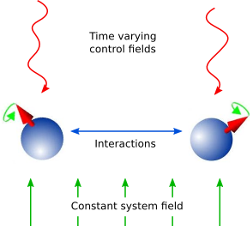
\includegraphics[width=0.5\linewidth]{principles_quantum_control.png}
    \caption{Schematic showing the principle of quantum control}
    \label{fig:principles_quantum_control}
\end{figure}

Here we will first consider only finite-dimensional, closed quantum systems.In closed quantum systems the states can be represented by kets, and the transformations on these states are unitary operators. 
The dynamics generators are Hamiltonians. The combined Hamiltonian for the system is given by
$$
H(t)=H_0+\sum_{j=1} u_j(t) H_j
$$
where $H_0$ is the drift Hamiltonian and the $H_j$ are the control Hamiltonians. The $u_j$ are time varying amplitude functions for the specific control.

The dynamics of the system are governed by Schrödingers equation.
$$
\frac{d}{d t}|\psi\rangle=-i H(t)|\psi\rangle
$$

Note we use units where $\hbar=1$ throughout. The solutions to Schrödinger's equation are of the form:
$$
|\psi(t)\rangle=U(t)\left|\psi_0\right\rangle
$$
where $\psi_0$ is the state of the system at $t=0$ and $U(t)$ is a unitary operator on the Hilbert space containing the states. 
$U(t)$ is a solution to the Schrödinger operator equation
$$
\frac{d}{d t} U=-i H(t) U, \quad U(0)=\mathbb{1}
$$

We can use optimal control algorithms to determine a set of $u_j$ that will drive our system from $\left|\psi_0\right\rangle$ to $\left|\psi_1\right\rangle$, this is state-to-state transfer, or drive the system from some arbitary state to a given state $\left|\psi_1\right\rangle$, which is state preparation, or effect some unitary transformation $U_{\text {target }}$, called gate synthesis. 
The latter of these is most important in quantum computation.

%%%%%%%%%%%%%%%%%%%%%%%%%%%%%%%
\subsection{GRAPE: Gradient Ascent Pulse Engineering}
The GRadient Ascent Pulse Engineering was first proposed in \cite{KHANEJA2005296}. 
Overview of GRAPE algorithm as implemented in QuTip is as follows. 
Solutions to Schrödinger's equation for a time-dependent Hamiltonian are not generally possible to obtain analytically. 
Therefore, a piecewise constant approximation to the pulse amplitudes is made. Time allowed for the system to evolve $T$ is split into $M$ timeslots (typically these are of equal duration), during which the control amplitude is assumed to remain constant. 

\begin{itemize}
    \item The combined Hamiltonian is approximated as: $H(t) \approx H\left(t_k\right)=H_0+\sum_{j=1}^M u_{j k} H_j$ \\
    where,  k is a timeslot index, 
            j is the control index, 
            and M is the number of controls. 
            Hence $t_k$ is the evolution time at the start of the timeslot, 
            and $u_{jk}$ is the amplitude of control j throughout timeslot k.
            Number of time steps $N=T/\delta t$.\\
    \item The time evolution operator, or propagator, within the timeslot can then be calculated as:  
            $U_k:=e^{-i H\left(t_k\right) \Delta t_k}$ \\
            where, $\Delta t_k$ is the duration of the timeslot.\\
            The evolution up to (and including) any timeslot k (including the full evolution k=M) can the be calculated as 
            $U\left(t_k\right):=U_k U_{k-1} \cdots U_1 U_0$
    \item A figure of merit or fidelity is some measure of how close the evolution is to the target, based on the control amplitudes in the timeslots. 
            The typical figure of merit for unitary systems is the normalised overlap of the evolution and the target. 
            See section \ref{sec:figure_of_merit} for details. 
    \item optimization pronlem and algorithm: 
        \begin{enumerate}
            \item There are now $N\times M$ variables to minimize the figure of merit. 
                The problem becomes a \underline{finite multi-variable optimization problem}.
            \item There are many established methods for this kind of problem. see section \ref{sec:finite_variables_optimization} for details. 
                The default method in the QuTiP Qtrl GRAPE implementation is the L-BFGS-B method in Scipy.
        \end{enumerate}
\end{itemize}

%%%%%%%%%%%%%%%%%%%%%%%%%%%%%%%
\subsection{CRAB: Chopped RAndom Basis}


\begin{enumerate}
    \item CRAB comes in when the pulse complexity is very low. \cite{PhysRevLett.106.190501}\cite{PhysRevA.84.022326} In such cases, it is sufficient to transform the optimal control problem to a few parameter search by introducing a physically motivated function basis that builds up the pulse. 
        Compared to the number of time slices needed to accurately simulate quantum dynamics (often equals basis dimension for Gradient based algorithms), this number is lower by orders of magnitude, 
        allowing CRAB to efficiently optimize smooth pulses with realistic experimental constraints. 
    \item choosing functional basis: 
        \begin{itemize}
            \item Consider a priori knowledge of the system \\
                $\rightarrow$ such as symmetries, magnitudes of scales,... \\
                $\rightarrow$ integrate experimental constraints such as maximum frequencies allowed, maximum amplitude, smooth ramping up and down of the pulse ...
            \item Consider expected solution (e.g. sign, smoothness, bang-bang behavior, singularities, maximum excursion or rate of change,....).
        \end{itemize}
    \item where CRAB differs from GRAPE: 
        \begin{itemize}
            \item Optimized pulse from CRAB is a smooth function.
            \item CRAB optimizes pulse function basis coefficient instead of amplitude of poulse at time slices.
            \item CRAB considers time slices only when calculating fidelity for a set of function basis coefficients. 
        \end{itemize}
    \item "dressed" CRAB: a variant of CRAB that is introduced in \cite{PhysRevA.92.062343} that allows to escape local minima. 
\end{enumerate}
%%%%%%%%%%%%%%%%%%%%%%%%%%%%%%%
\subsection{Figure of merit, cost function}\label{sec:figure_of_merit}
state transfer case
single-state state transfer: 
\begin{align*}
    f(\vec{\epsilon}(t)) &= \mathcal{F}(\vec{\epsilon}(t)) \quad \text{state fidelity}\\
    &\equiv \abs{\bra{\psi_{targ}} U(T,\vec{\epsilon}(t)) \ket{\psi_{init}}}^2 \\
    &= \abs{\bra{\psi_{targ}} 
        \mathcal{T}\exp{-\frac{i}{\hbar}\int_0^T dt H(\vec{\epsilon}(t))}
        \ket{\psi_{init}}}^2 \\
    &\text{make the problem numerical, make $\vec{\epsilon}(t)$ a piece-wise constant function with $N=T/\delta t$,} \\
    &\text{$\delta t$ is a parameter, usually set to time resolution of AWG.} \\
    &= \abs{\bra{\psi_{targ}} 
        U_NU_{N-1}...U_1
        \ket{\psi_{init}}}^2, \quad \text{where, } U_k=\exp{\frac{i\delta t}{\hbar}H(\vec{\epsilon}(k\delta t))} \\
\end{align*}

multi-state state transfer:
\begin{align*}
    f(\vec{\epsilon}(t)) &= \mathcal{F}(\vec{\epsilon}(t)) \quad \text{Fidelity}\\
    &\equiv 
        \begin{cases}
            \abs{\sum_k \bra{\psi_{targ}^{(k)}} U(T,\vec{\epsilon}(t)) \ket{\psi_{init}^{(k)}}}^2 &\text{coherent} \\
            \sum_k \abs{\bra{\psi_{targ}^{(k)}} U(T,\vec{\epsilon}(t)) \ket{\psi_{init}^{(k)}}}^2 &\text{inoherent}
        \end{cases} \\
    &\text{for coherent case with number of state = dimension of Hilbert space,}\\
    &=\abs{\text{Tr}\left[U(T,\vec{\epsilon}(t))U_{targ}^{\dagger}\right]}^2 \quad \text{unitary fidelity}\\
\end{align*}

%%%%%%%%%%%%%%%%%%%%%%%%%%%%%%%
\subsection{Finite variables optimization algorithms}\label{sec:finite_variables_optimization}
\begin{equation}
    H(\vec{\epsilon}(t)) = H_0 + \sum_{k=1}^m \epsilon_k(t) H_k
\end{equation}
Goal: Find optimal control field $\vec{\epsilon}(t)$ that optimizes some function $f(\vec{\epsilon}(t)) = f(H(\vec{\epsilon}(t)))$. \\
\\
Procedure: 
\begin{enumerate}
    \item To optimize a large number of parameters, we need:
        \begin{enumerate}
            \item an efficient means of calculating the gradients of cost function w.r.t parameters
            \item sub-optial local minima are sufficiently unlikely or close to global minima
        \end{enumerate}
    \item Given methods to calculate cost function and gradients, we have two main classes of algorithm for performing optimization: 
        \begin{itemize}
            \item line-search methods: one alternates between picking a direction in parameter space, radiating from our current point, and subsequently performing a 1-d minimization protocol to find the minimum along this line. \\
                $\rightarrow$ basic gradient descent: choose direction as gradient at the point. \\
                $\rightarrow$ Newton method: choose direction using both gradient and Hessian matrix at the point. $\rightarrow$ quasi-Newton, L-BFGS
            \item trust-region methods
        \end{itemize}
    \item calcualte gradient of $f(\vec{\epsilon}(t))$ with respect to $\vec{\epsilon}(t)$
        \begin{enumerate}
            \item For an analytical function $f(\vec{\epsilon})$, gradient is given by $\nabla f(\vec{\epsilon}) = \sum_{i=1}^m \frac{\partial f(\vec{\epsilon})}{\partial \epsilon_i} \hat{\epsilon}_i$
            \item For discrete $\vec{\epsilon}$, gradient of $f(\vec{\epsilon})$ is given by the finite difference method.
            \item approximate the gradient: skipping here.
            \item When calculating / approximating gradient is too expensive, cosider optimization algorithm other than gradient descent.
        \end{enumerate}
    \item take a step (step size as a parameter) in the direction. \\
        step size too small: optimization takes long\\
        step size too large: may never reach true optima
    \item calcualte gradient again
    \item repeat until convergence
\end{enumerate}


%%%%%%%%%%%%%%%%%%%%%%%%%%%%%%%
\subsection{Pulse constraints}
\begin{enumerate}
    \item constraints come from AWG(Arbitrary Wave Generator)'s amplitude and bandwidth constraints
        $\rightarrow$ consider adding a set of constraint terms to the cost function
        \begin{equation*}
            f(\vec{\epsilon}(t)) = \mathcal{F}(\vec{\epsilon}(t)) + \sum_i \lambda_i g_i(\vec{\epsilon})
        \end{equation*}
    \item pulse amplitude: the output power of our AWG is limited, and thus to be feasible, we need $\epsilon(t) \le \epsilon_{max}$ for all t. $\rightarrow$ hard cutoff / soft cutoff
        \begin{enumerate}
            \item Employ an optimization algorithm which naturally allows for such constraints $\rightarrow$ see K-BFGS-B in scipy.optimize
            \item Parametrise optimization problen 
                \begin{align*}
                    &\stackrel{\text{maximize}}{\vec{\epsilon}(t)}  \mathcal{F} (\vec{\epsilon}(t)) 
                    \rightarrow \stackrel{\text{maximize}}{\vec{x}}  \mathcal{F} (\vec{\epsilon}(\vec{x})) \\
                    &\text{where, } \epsilon_k = \epsilon_{max} \tanh{(x_k)} 
                \end{align*}
        \end{enumerate}
    \item pulse bandwidth:   
        \begin{itemize}
            \item soft cutoff
            \item hard cutoff
            \item linear frequency-dependent penalty
        \end{itemize}
\end{enumerate}

\subsubsection{Pulse constraint: limiting the intermediate photon number}
Since computer memory is finite, we are forced to choose a photon number truncation nph such that the operator a becomes a $n_{ph} \times n_{ph}$ matrix. 
When we do this, we are in effect replacing our infinite-dimensional oscillator with a finite-dimensional qudit. 
This replacement is only valid if all of the system dynamics relevant for the desired state transfers occurs within the $\{\ket{0} ,\cdots , \ket{n_{ph} - 1} \}$ subspace. 
For generic applied drives this is not the case. In order to enforce this property, we modify the optimization problem to find a solution which operates identically under several different values of $n_{ph}$.
Writing the fidelity as computed with a truncation nph as $F_{n_{ph}}$, we have:
\begin{equation}
    \stackrel{\text{maximize}}{\vec{\epsilon}} \left( \sum_k F_{n_{ph}+k} (\epsilon(t)) \right) - \left( \sum_i \lambda_i g_i (\epsilon(t)) \right)
\end{equation}

\begin{itemize}
    \item To enforce that the behavior is identical in the different truncations, we add the penalty term: 
        \begin{equation*}
            g_{\text {discrepancy }}(\boldsymbol{\epsilon}(\boldsymbol{t}))=\sum_{k_1 \neq k_2}\left(\mathcal{F}_{n_{\mathrm{ph}}+k_1}(\boldsymbol{\epsilon}(t))-\mathcal{F}_{n_{\mathrm{ph}}+k_2}(\boldsymbol{\epsilon}(t))\right)^2
        \end{equation*}
        I think it's making the cost function symmetrical w.r.t. $n_{ph}$.
    \item A more recently developed, and more direct, method is to add a penalty term for any occupation of the final photon state ($\ket{n_{ph} - 1}$) in the truncated Hilbert space at any time:
        \begin{equation*}
            g_{\text {trajectory }}=\sum_{k=1}^N\left|\left\langle n_{\text {ph }}-1 \mid \psi_{\text {fwd }}^{(k)}\right\rangle\right|^2
        \end{equation*}
\end{itemize}

\subsection{Troubleshooting optimization convergence}
Check list: 
\begin{enumerate}
    \item Check that the time given $T = N \delta t$ is appropriate.
        \begin{itemize}
            \item Specified in units that are consistent with the units specifying the Hamiltonian. For instance, if the Hamiltonian is specified in GHz, then the time step should be in units of ns.
            \item N value appropriate
        \end{itemize}
    \item check constraints
        \begin{itemize}
            \item Completely remove all constraints and penalties, and make sure that the algorithm works in this context before re-introducing them
        \end{itemize}
    \item check algorithm 
        \begin{itemize}
            \item check termination conditions \\
            Gradient based search algorithms usually have termination conditions specified in terms of the norm of the gradient. It is often necessary to lower the gradient norm threshold for termination to ensure that it does not give up -> gtol in scipy.minimize

        \end{itemize}
    \item check ionitial guess
        \begin{itemize}
            \item Avoid special initial guesses, this depends on the algorithm. 
                For gradient-based algo, make sure initial gradient is not vanishing.
        \end{itemize}
    \item miscellaneous checks
        \begin{itemize}
            \item Truncation of cavity-state Hilbert space large enough? 
        \end{itemize}
\end{enumerate}

%%%%%%%%%%%%%%%%%%%%%%%%%%%%%%%%%%%%%%%%%%%%%%%%%%%%%%%%%%%%%%%
\section{State preparation pulse optimization}
All codes mentioned in this section are available in the GitHub repository \cite{lzl_github_repo}.

%%%%%%%%%%%%%%%%%%%%%%%%%%%%%%%
\subsection{Starting with a simple diagnostic pulse, single qubit system}
To verify that I have a working code that can optimize a pulse, 
I will start with a simple qubit flip operation of a single-qubit system.
The purpose of this section is to show that the algorigm is indeed running optimization
by recovering analytically solvable state-to-state transer using pulse optimization. 
\\
In the following example, we consider using the CRAB algorithm as implemented in the 
qutip python library. In qutip, the ctrlpulseoptim.optimize\_pulse\_unitary function is used 
to optimize pulse shapes to minimize the fidelity error, which is equivalent maximising the fidelity to an optimal value of 1.
\\
The Hamiltonian of a single qubit system with arbitrary control is give by, 
\begin{equation}
    H(t) = \frac{\hbar \omega_0}{2} \sigma_z + \epsilon_x(t)\sigma_x + \epsilon_y(t)\sigma_y 
\end{equation}
where, $\epsilon_x(t), \epsilon_y(t)$ are control pulses.  
\\
Consider a special case of the above general case. 
\begin{equation}
    H_1(t) = \frac{\hbar \omega_0}{2} \sigma_z + \frac{\hbar \omega_1}{2}(\sigma_x\cos{\omega t} + \sigma_y\sin{\omega t})    
\end{equation}

% TODO: add derivation here
From Valerio's note, via frame rotation, starting from $\ket{\psi_{init}} = \ket{+\hat{z}}$, 
we have evoloved state, 
\begin{equation}
    |\psi(t)\rangle=e^{-i \omega t / 2}[\cos (\Omega t / 2)-i \cos \theta \sin (\Omega t / 2)]|+\hat{z}\rangle-i e^{i \omega t / 2} \sin \theta \sin (\Omega t / 2)|-\hat{z}\rangle
\end{equation}
where, 
$$
\Omega=\sqrt{\left(\omega_0-\omega\right)^2+\omega_1^2} \\
\cos \theta=\frac{\omega_0-\omega}{\Omega}
$$

Suppose we want to achieve a state-to-state transfer from $\ket{+\hat{z}}$ to $\ket{-\hat{z}}$,  
$$
P_{+\hat{z} \rightarrow-\hat{z}}(t) = \sin ^2 \theta \sin ^2(\Omega t / 2)=\left(\frac{\omega_1}{\Omega}\right)^2 \sin ^2(\Omega t / 2)
$$
With $H_1(t)$, $P_{+\hat{z} \rightarrow-\hat{z}}(t)$ only goes to 1 if 
\begin{enumerate}
    \item $\omega_1 = \Omega$, i.e. $\omega = \omega_0$.
    \item $\omega_1 = \frac{\pi}{T}$ (with evolution time T fixed, smallest frequency needed)
\end{enumerate}
\\
Now we run the pulse optimization and compare with analytical result. 
\\
Let t = evo\_time = T
\\
Defining the time evolution parameters:
- To solve the evolution the control amplitudes are considered constant within piecewise timeslots, hence the evolution during the timeslot can be calculated using U(t\_k) = expm(-iH(t\_k)dt). 
- Combining these for all the timeslots gives the approximation to the evolution from an initial state ψ0 at t=0 to U(T)ψ0 at the t=evo\_time. The number of timeslots and evo\_time have to be chosen such that the timeslot durations (dt) are small compared with the dynamics of the system.
- set drift frequency $\omega_0$ to some number, at resonance $\omega = \omega_0$, for state to state transfer to happen at the end of pulse, require $\omega_1 = \frac{\pi}{T}$.
\\
Next, we set the initial guess pulses where the pulse optimization algorithm starts. 
During the each iteration of the optimization, the Nelder-Mead algorithm calculates a new set of coefficients that improves the currently worst set among all set of coefficients. For details see [1,2] and a textbook about static search methods. 
The algorithm continues until one of the termination conditions defined above has been reached. If undesired results are achieved, rerun the algorithm and/or try to change the number of coefficients to be optimized for, as this is a very crucial parameter.  

% TODO: add here the results from GRAPE and CRAB, and discuss their issues with the intended goal\
The optimized pulses are: 
\begin{figure}[H]
    \centering
    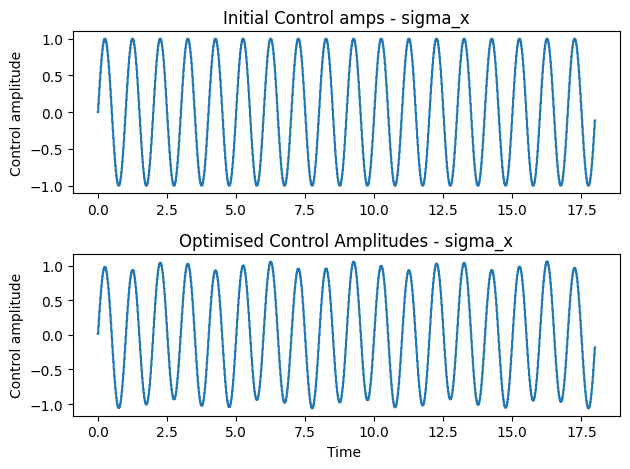
\includegraphics[width=0.95\linewidth]{single_qubit_control1.png}
    \caption{single qubit control 1 pulse}
    \label{fig:single_qubit_control1}
\end{figure}
\begin{figure}[H]
    \centering
    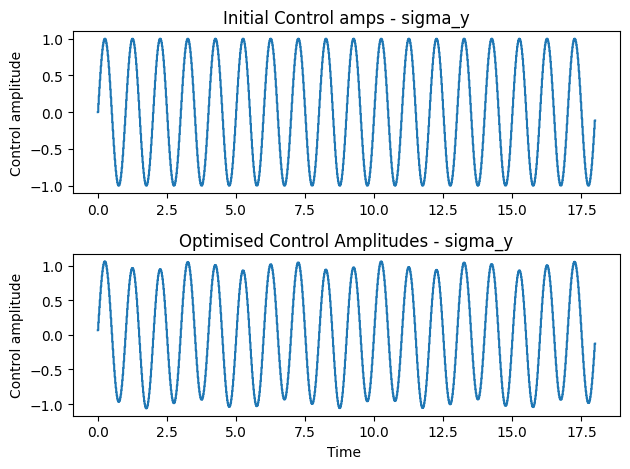
\includegraphics[width=0.95\linewidth]{single_qubit_control2.png}
    \caption{single qubit control 2 pulse}
    \label{fig:single_qubit_control2}
\end{figure}

Though the exact analytical solution couldn't be recovered from from numetical optimization, 
the algorithm can be crudely verified to be running by a crude self-implemented forward 
evolution simulation code snippet. 

% TODO: describe the simple self-implemented forward simulation code here and add graphs

% TODO: add the code in annex and add link to github

% TODO: discuss why is there a qutip simulation and a self-implemented simulation

%%%%%%%%%%%%%%%%%%%%%%%%%%%%%%%
\subsection{Diagnostic pulse: cavity vacuum to cavity coherent state}
Having tested the code on a single qubit system, we now move on to a more complex system that I am eventually interested in. 
In this code, we consider a cavity coupled to a single qubit.
%TODO:
% - revise Reinhold thesis
% - vet the following section with chiyuan, 几个哈密度量的物理意义 + 他们之间的转换  
% - discuss that we are just looking at area under curve here, code to calcualte area under curve
For this physical system, we have drift Hamiltonian, 
from Reinhold PhD thesis (2.13) \cite{reinhold2019}: 
\begin{equation}
    H_d = \omega_q a^\dagger a + \frac{\omega_z}{2} \sigma_z + \frac{\chi}{2} a^\dagger a \sigma_z
\end{equation}
It can be shown that it's equivalent to: %TODO: vet this
\begin{equation}
    \begin{aligned}
    H_d &= g\left( \hat{\sigma}_+ \hat{\sigma}_- + \hat{a}^{\dagger}\hat{a}\hat{\sigma}_z \right) \\
    &= g \left( \frac{1}{2}(1+\hat{\sigma}_x) + \hat{n}\hat{\sigma}_z\right)
\end{aligned}
\end{equation}

where, $g$ is the cavity-qubit coupling strength which is set to be $50*2 \pi MHz$ here, as given by experiment
% TODO: ask chiyuan about g value, cite paper for this valu 
\\
For this physical system we have both cavity and auxiliary qubit contorl, in the form of control Hamiltonian: 
\begin{equation}
    H_c = \epsilon_c(t) \hat{a} + \epsilon_T(t) \hat{\sigma}_- + h.c.
\end{equation}

where, 
\begin{itemize}
    \item $\epsilon_c(t)$ is the contorl signal to cavity
    \item $\epsilon_T(t)$ is the control signal to ancilliary qubit
\end{itemize} 

with $\hat{\sigma}_- = \frac{1}{2} \hat{\sigma}_x - \frac{i}{2}\hat{\sigma}_y$, 
rewrite $H_c$ as following for ease of implementation using QuTip:
\begin{equation}
    H_c = \epsilon_c(t) \hat{a} + \epsilon_T(t) (\frac{1}{2} \hat{\sigma}_x - \frac{i}{2}\hat{\sigma}_y) + h.c.
\end{equation}
Assuming that the control signals $\epsilon_c(t), \epsilon_T(t)$ are real, and ignoring scalar constants, we have 
$$
H_c = \epsilon_c(t) (\hat{a}+\hat{a}^{\dagger}) + \epsilon_T(t) \hat{\sigma}_x
$$

Initial and target states: 
\begin{equation}
    \begin{aligned}
    \ket{\psi_{\text{initial}}} &= \ket{\alpha} \\
    \ket{\psi_{\text{final}}} &= \ket{\alpha} + \ket{-\alpha}
\end{aligned}
\end{equation}


For testing the code, consider
\begin{equation}
    \begin{aligned}
        \ket{\psi_{\text{initial}}} &= \ket{0} \\
        \ket{\psi_{\text{final}}} &= \ket{\alpha}
    \end{aligned}
\end{equation}


The optimization algorithm settings used in this example are: 
\begin{itemize}
    \item Number of time slots, n\_ts = 100
    \item Time allowed for the evolution, evo\_time = 1
    \item Fidelity error target, fid\_err\_targ = 1e-4
    \item Maximum iterations for the optisation algorithm, max\_iter = 100000
    \item Maximum (elapsed) time allowed in seconds, max\_wall\_time = 10000
    \item optimization algorithm: GRAPE
\end{itemize}

The initial and optimised pulses:

\begin{figure}[H]
    \centering
    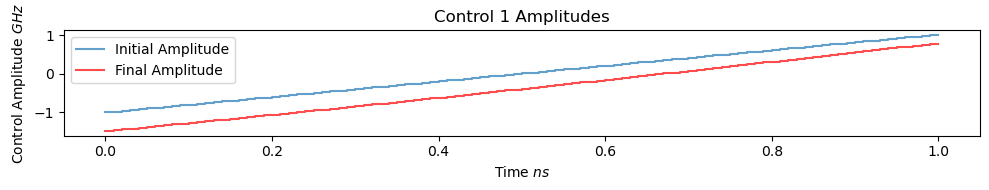
\includegraphics[width=0.95\linewidth]{vac2coherent_control1.png}
    \caption{vacuum to coherent control 1 pulse}
    \label{fig:vac2coherent_control1}
\end{figure}
\begin{figure}[H]
    \centering
    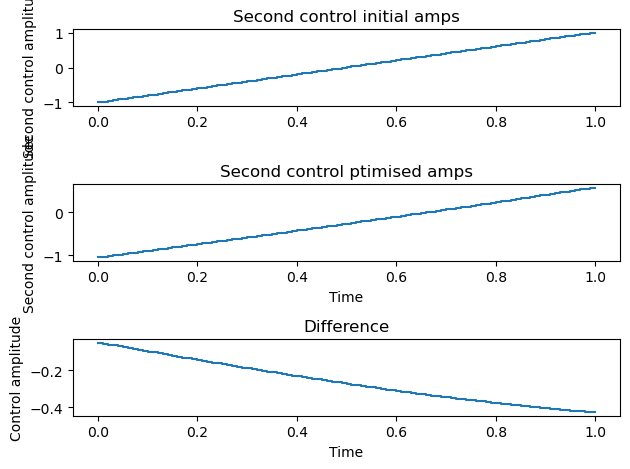
\includegraphics[width=0.95\linewidth]{vac2coherent_control2.png}
    \caption{vacuum to coherent control 2 pulse}
    \label{fig:vac2coherent_control2}
\end{figure}

Forward simulation is as follows: 
\begin{figure}[H]
    \centering
    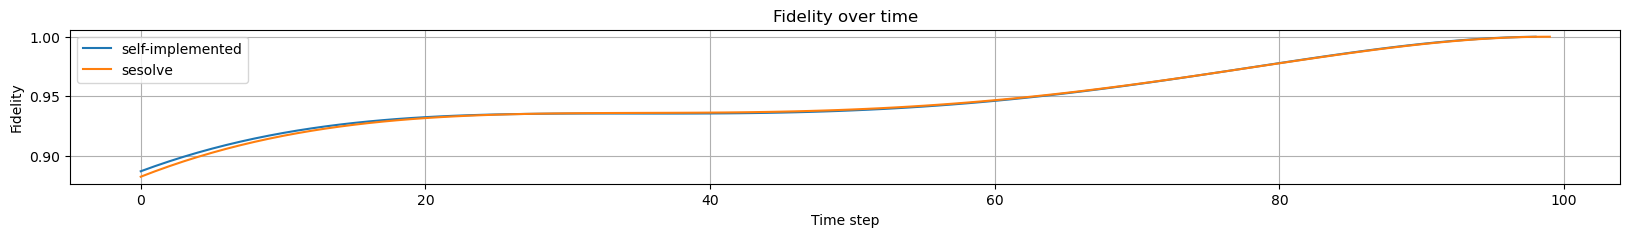
\includegraphics[width=0.95\linewidth]{vac2coherent_simulate.png}
    \caption{vacuum to coherent forward simulate}
    \label{fig:vac2coherent_simulate}
\end{figure}

To verify whether the cavity state basis truncation $N$ is large enough, i.e. 
whether the optimziation result has converged with respect to $N$, consider: 
\begin{enumerate}
    \item Run the optimization with the same algorithm settings and same initial guess, but with different $N$ values. 
        Then plots the optimized pulses ran with different $N$ values on the same plot. 
    \item Simulate the evolution of the system with the optimized pulses, but with a range of higher $N$ values. 
\end{enumerate}

\begin{figure}[H]
    \centering
    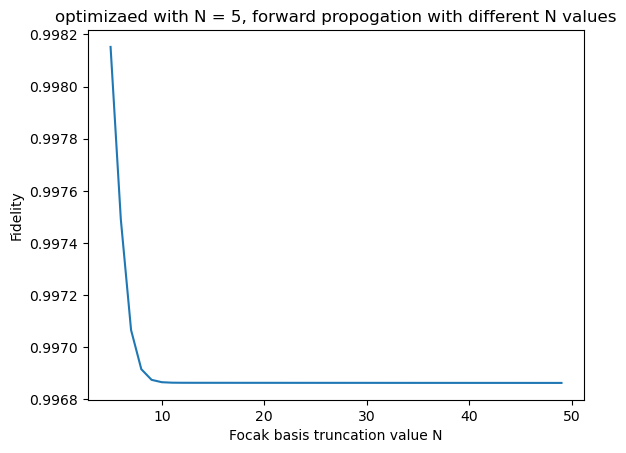
\includegraphics[width=0.95\linewidth]{vac2coherent_N_convergence.png}
    \caption{cavity state Fock basis truncation $N$ convergence}
    \label{fig:vac2coherent_N_convergence}
\end{figure}

\begin{figure}[H]
    \centering
    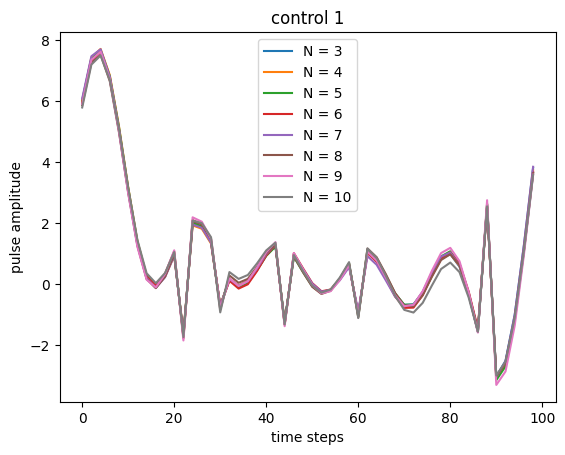
\includegraphics[width=0.95\linewidth]{check_convergence_control1.png}
    \caption{cavity state Fock basis truncation $N$ convergence}
    \label{fig:check_convergence_control1}
\end{figure}

\begin{figure}[H]
    \centering
    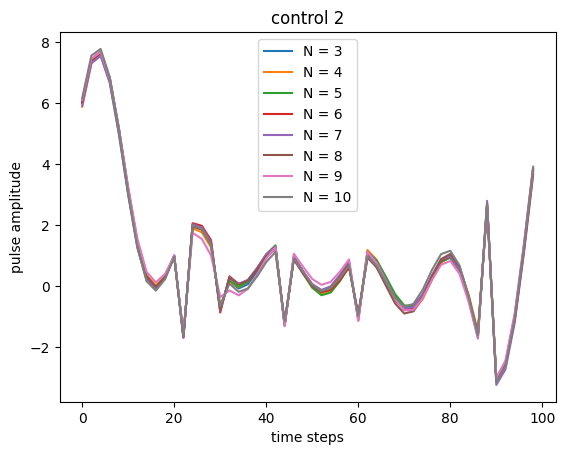
\includegraphics[width=0.95\linewidth]{check_convergence_control2.png}
    \caption{cavity state Fock basis truncation $N$ convergence}
    \label{fig:check_convergence_control2}
\end{figure}

%%%%%%%%%%%%%%%%%%%%%%%%%%%%%%%
\subsection{Diagnostic pulse: unselective spin flip, cavity coupled with single qubit(effective)}
Going from a cavity cavuum state to a cavity coherent state analytically requires only a displacement operation
which requires only a control pulse to the cavity. Hence, in the previous disagnostic scenario the full Hamiltonia
with all three (real) control channels were not used.
\\
Here we consider the full system Hamiltonian (cavity + auxiliary qubit + coupling terms)
drift Hamiltoinan is given by, 
\begin{equation}
    H_d = \text{wr} * n_{\text{cavity}} + \text{Ez} * \sigma_z + \text{chi} * \sigma_z * (n_{\text{cavity}} + 1/2 )    
\end{equation}
where parameters of the physical system are:
\\
(notet that energy terms have unit $GHz$ and time terms have unit $ns$)
% TODO: ask chiyuan how to get these numbers
\begin{itemize}
    \item cavity frequency, wr = $2 \pi$
    \item qubit anharmonicity Ez = $0.44 \pi$
    \item qubit-cavity coupling strength chi = $0.007$
\end{itemize}

Real control channels in the Hamiltonain are given by (each term comprises a channel): 
\begin{equation}
    H_c = a + a^{\dagger} + -1j*(a - a^{\dagger}) + \sigma_x    
\end{equation}

The initial and target states for this pulse optimization code are: 
\begin{align*}
    \psi_0 &= \frac{1}{\sqrt{2}} (\ket{0}_{\text{cavity}} \otimes \ket{0}_{\text{qubit}} 
                + \ket{1}_{\text{cavity}} \otimes \ket{0}_{\text{qubit}})\\
    \psi_{\text{targ}} &= \frac{1}{\sqrt{2}} (\ket{0}_{\text{cavity}} \otimes \ket{1}_{\text{qubit}} 
                + \ket{1}_{\text{cavity}} \otimes \ket{1}_{\text{qubit}})\\
\end{align*}

where the qubit state is flipped irrepsective of the cavity state
\\
The final optimization algorithm parameters are:
\\ 
%TODO: ask chiyuan how the appropriate pulse length is calcualted
\begin{itemize}
    \item optimization algorithm: GRAPE
    \item Number of time slots, n\_ts = 500
    \item Time allowed for the evolution, evo\_time = 1
    \item Fidelity error target, fid\_err\_targ = 1e-3
    \item Maximum iterations for the optisation algorithm, max\_iter = 1000
    \item Maximum (elapsed) time allowed in seconds, max\_wall\_time = 120
    \item initial guess pulse type, p\_type = 'LIN'
\end{itemize}

The inital and optimized pulses are: 
\begin{figure}[H]
    \centering
    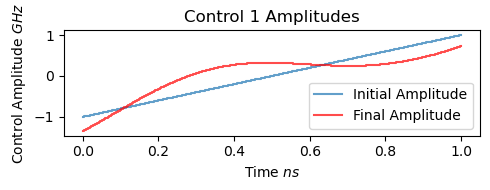
\includegraphics[width=0.95\linewidth]{unselective_spin_flip_control1.png}
    \caption{unselective spin flip control 1 pulse amplitudes}
    \label{fig:unselective_spin_flip_control1}
\end{figure}
\begin{figure}[H]
    \centering
    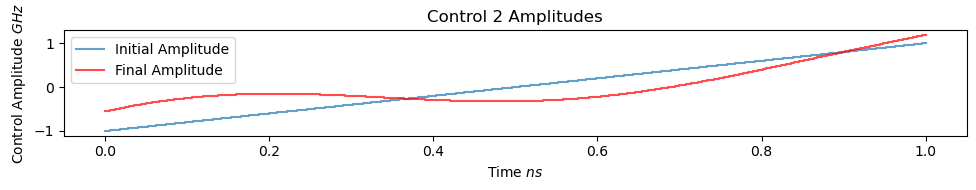
\includegraphics[width=0.95\linewidth]{unselective_spin_flip_control2.png}
    \caption{unselective spin flip control 2 pulse amplitudes}
    \label{fig:unselective_spin_flip_control2}
\end{figure}
\begin{figure}[H]
    \centering
    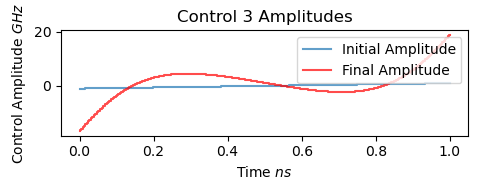
\includegraphics[width=0.95\linewidth]{unselective_spin_flip_control3.png}
    \caption{unselective spin flip control 3 pulse amplitudes}
    \label{fig:unselective_spin_flip_control3}
\end{figure}

Forward simulation is given below to ensure that pulse optimization has run properly. 
\\
Simulation gives: 
\begin{itemize}
    \item sesolve final fidelity:  0.9995869703894827
    \item self-implemented final fidelity:  0.9995575205270999
\end{itemize}
\begin{figure}[H]
    \centering
    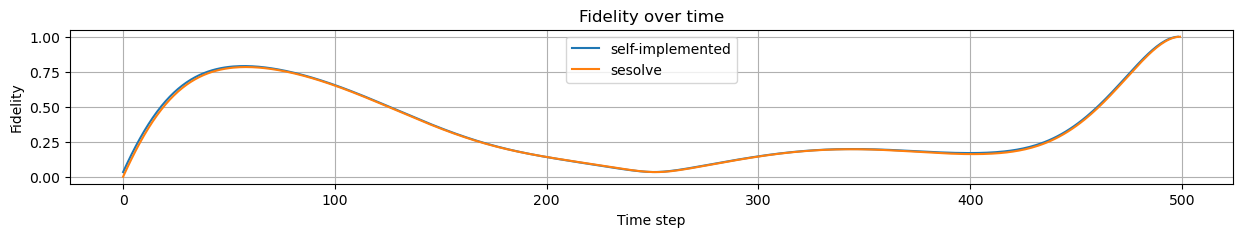
\includegraphics[width=0.95\linewidth]{unselective_spin_flip_simulation.png}
    \caption{unselective spin flip forward simulation}
    \label{fig:unselective_spin_flip_forward_simulation}
\end{figure}

%%%%%%%%%%%%%%%%%%%%%%%%%%%%%%%
\subsection{Diagnostic pulse: selective spin flip, cavity coupled with single qubit(effective)}

For this scenario, the drift and contorl Hamiltonian terms are same as in the previous section. We are interested in this state 
preparation because as achieved by Krastanov et al.(2015) \cite{Krastanov2015} which gave a contruction for how to achieve arbitrary 
operation on dispersively coupled cQED systems using a set of two opeartions: displacements and selective number-dependent arbitrary phase (SNAP) operations. 
SNAP operations allow an arbitrary set of relative phases to be applied to different photon number states, and can be represented with the form
\begin{equation}
    S(\vec{\theta}) = \sum_k e^{i\theta_k} \ket{k}\bra{k}
\end{equation}

Clearly, SNAP operations require selective spin rotations of which selective spin flip is a special case.
\\
State preparation optimization target is as follow: 
\begin{align*}
    \psi_0 &= \frac{1}{\sqrt{2}} (\ket{0}_{\text{cavity}} \otimes \ket{0}_{\text{qubit}} 
                + \ket{1}_{\text{cavity}} \otimes \ket{0}_{\text{qubit}})\\
    \psi_{\text{targ}} &= \frac{1}{\sqrt{2}} (\ket{0}_{\text{cavity}} \otimes \ket{0}_{\text{qubit}} 
                + \ket{1}_{\text{cavity}} \otimes \ket{1}_{\text{qubit}})\\
\end{align*}
(where qubit spin flip is selective on cavity state)
% TODO: 问chiyuan,selective spin flip 和 unselective spin flip 的主要区别在哪
% discuss 
% - selective spin flip 和 unselective spin flip 的主要区别在哪
% - why is selective spin flip the next step
% - discuss pulse amplitude constraint
% - ask chiyuan how the appropriate pulse length is calcualted
% - figure out about the cavity state going to higher photon number state inbetween state transition

\\

The best optimization result that was obtained by tuning the optimization script from 
previous section is as follow. 
\\
The final optimization algorithm parameters are:
\\ 
\begin{itemize}
    \item optimization algorithm: GRAPE
    \item Number of time slots, n\_ts = 100000
    \item Time allowed for the evolution, evo\_time = 500
    \item Fidelity error target, fid\_err\_targ = 1e-8
    \item Maximum iterations for the optisation algorithm, max\_iter = 10000
    \item Maximum (elapsed) time allowed in seconds, max\_wall\_time = 7200
    \item initial guess pulse type, p\_type = 'SINE'
\end{itemize}

The inital and optimized pulses are: 
\begin{figure}[H]
    \centering
    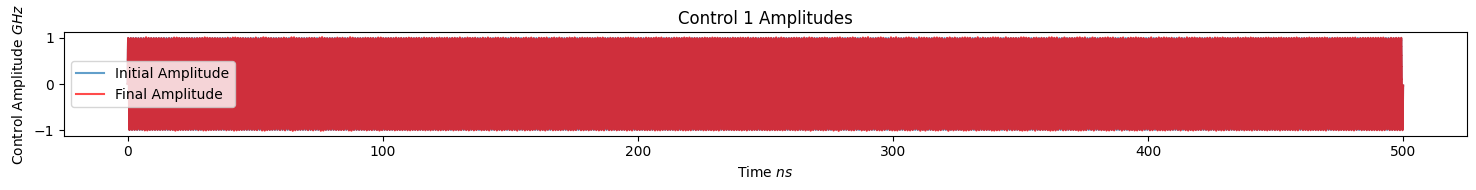
\includegraphics[width=0.95\linewidth]{selective_spin_flip_GRAPE_control1.png}
    \caption{selective spin flip control 1 pulse amplitudes}
    \label{fig:selective_spin_flip_control1}
\end{figure}
\begin{figure}[H]
    \centering
    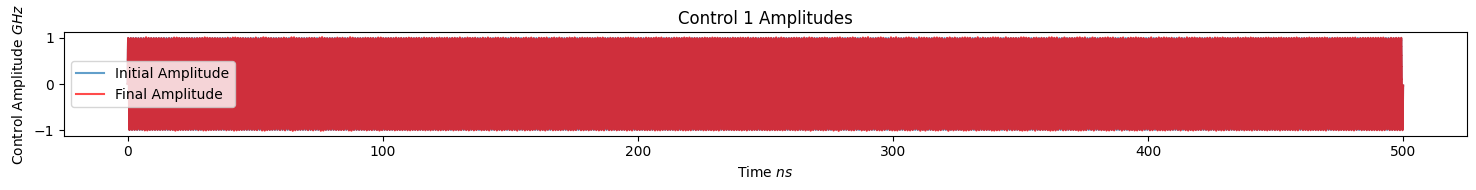
\includegraphics[width=0.95\linewidth]{selective_spin_flip_GRAPE_control1.png}
    \caption{selective spin flip control 2 pulse amplitudes}
    \label{fig:selective_spin_flip_control2}
\end{figure}
\begin{figure}[H]
    \centering
    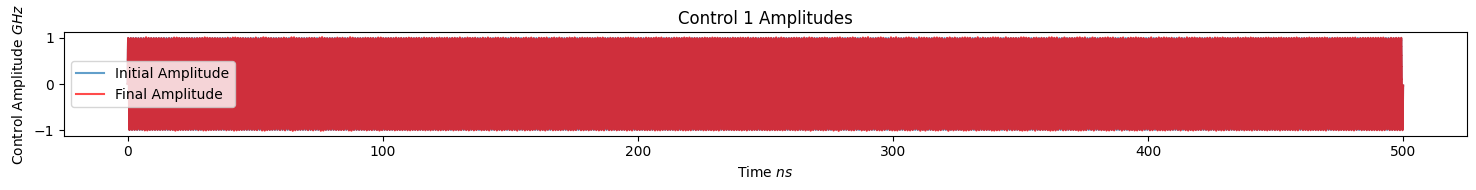
\includegraphics[width=0.95\linewidth]{selective_spin_flip_GRAPE_control1.png}
    \caption{selective spin flip control 3 pulse amplitudes}
    \label{fig:selective_spin_flip_control3}
\end{figure}

The control pulses have very fast oscillations due to the large number of time slices.
Zooming into control 1 pulse amplitudes, as shown in fig \ref{fig:selective_spin_flip_control3_zoomin},
we see that the pulse is fairly smooth. However, this fast oscillation is still not desirable and preferably gotten rid of. 
Another reason that might have contributed to this fast oscillation is the background frequency of the cavity and qubit 
of which the control pulses are trying to cancel out. One way to partially deal with this fast oscillation issue is to work
with the Hamiltonian in the rotating frame which will be tried out in the next section when cavity vacuum state to cavity cat state
is being optimized.  

Forward simulation is given below to ensure that pulse optimization has run properly. 
\\
Simulation gives: 
\begin{itemize}
    \item sesolve final fidelity:  0.9994876128337873
    \item cavity ptrace fidelity:  0.9997184822307845
    \item qubit ptrace fidelity:  0.999999719275808
    \item self-implemented final fidelity:  0.9997005493228243
\end{itemize}
\begin{figure}[H]
    \centering
    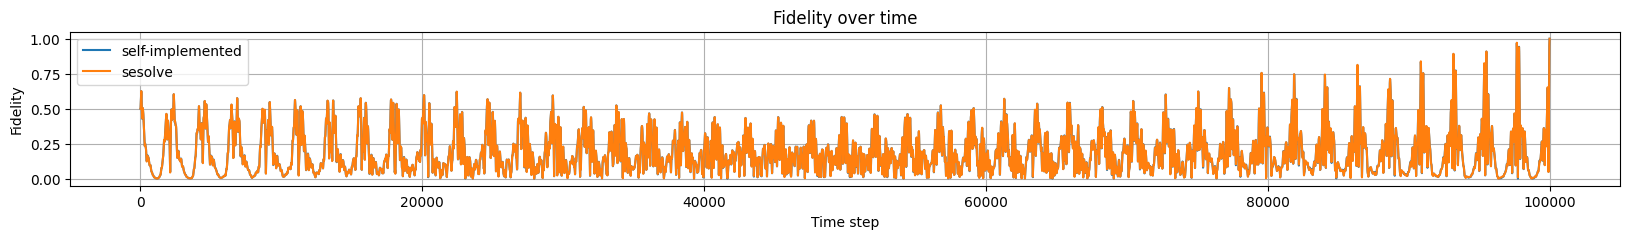
\includegraphics[width=0.95\linewidth]{selective_spin_flip_GRAPE_simulation.png}
    \caption{selective spin flip forward simulation}
    \label{fig:selective_spin_flip_forward_simulation}
\end{figure}


A particular analytical solution as given by Chiyuan already gives fidelity of $~0.98$.
            We expect a higher fidelity from a numerical optimization solution. 
            % TODO: ask chiyuan for analytical solution and put here
\\
However, this numerical solution has the folowing issues.
The optimzied pulses go beyong the amplitude constrains that required for the effective Hamiltonian to be valid. 
When the pulse amplitdes constrained are supplied to the optimziation algorithms, the results are not very satisfactory. 
% TODO: try the code with pulse amplitude constraints}
\\
The following run has two modifications: 
\begin{itemize}
    \item initial guess pulse is changed from sindusoidal to linear to see whether this improves the fast oscillation issue
    \item Pulse amplitude constraints are added to the optimization algorithm
\end{itemize}
However, as can be seen from the optimized pulses below, the fast oscillation issue is not resolved well. 
This is especially so for control 3.
\\

The inital and optimized pulses are: 
\begin{figure}[H]
    \centering
    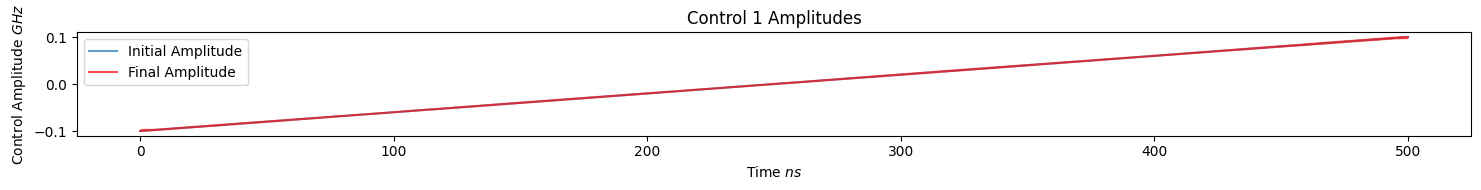
\includegraphics[width=0.95\linewidth]{selective_spin_flip_GRAPE_500,_100_000_LIN_constraints_control1.png}
    \caption{selective spin flip control 1 pulse amplitudes}
    \label{fig:selective_spin_flip_constrains_control1}
\end{figure}
\begin{figure}[H]
    \centering
    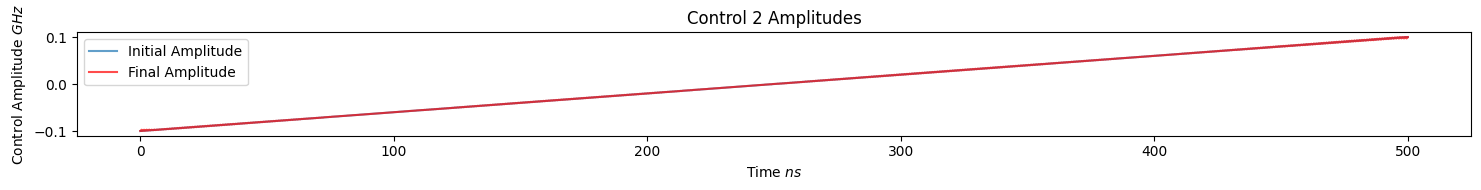
\includegraphics[width=0.95\linewidth]{selective_spin_flip_GRAPE_500,_100_000_LIN_constraints_control2.png}
    \caption{selective spin flip control 2 pulse amplitudes}
    \label{fig:selective_spin_flip_constrains_control2}
\end{figure}
\begin{figure}[H]
    \centering
    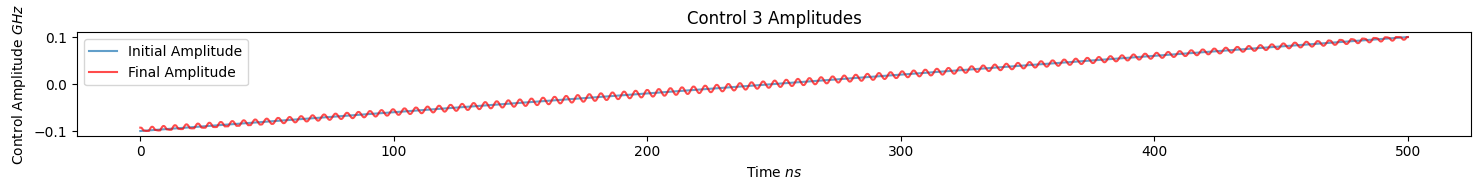
\includegraphics[width=0.95\linewidth]{selective_spin_flip_GRAPE_500,_100_000_LIN_constraints_control3.png}
    \caption{selective spin flip control 3 pulse amplitudes}
    \label{fig:selective_spin_flip_constrains_control3}
\end{figure}

Forward simulation is given below to ensure that pulse optimization has run properly. 
\\
Simulation gives: 
\begin{itemize}
    \item sesolve final fidelity:  0.9992259750482354
    \item cavity ptrace fidelity:  0.9992525011412332
    \item qubit ptrace fidelity:  0.9992706948956261
    \item self-implemented final fidelity:  0.9999937323329505
\end{itemize}
\begin{figure}[H]
    \centering
    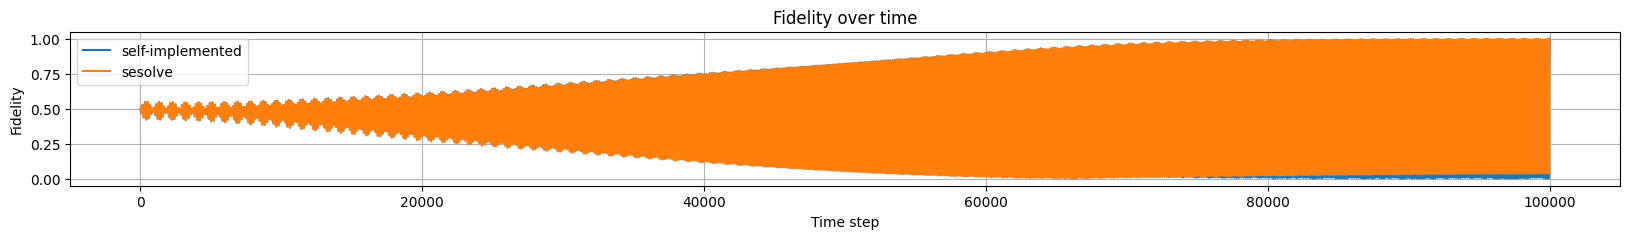
\includegraphics[width=0.95\linewidth]{selective_spin_flip_GRAPE_500,_100_000_LIN_constraints_simulation.png}
    \caption{selective spin flip forward simulation}
    \label{fig:selective_spin_flip_constraints_forward_simulation}
\end{figure}

At this point, we continued varying the parameters (puse length, number of slices, initial guess pulse, etc.). 
However, none gave optimization results where fidelity, pulse amplitude, pulse smoothness and fast oscillation issue 
are all accounted for satisfactorily. 

%%%%%%%%%%%%%%%%%%%%%%%%%%%%%%%
\subsection{vacuum to cat state, cavity coupled with single qubit(effective)}
In this section, we finally get to do a state preparation optimization of cavity vacuum state to cavity cat state.
The most efficient way to do this is to optimize for the cavity state alone by tracing out the qubit state when calculating state fidelity. 
However, the QuTip package does not support this feature. I attemped to modify QuTip source code to allow for this feature but failed. 
One might naively think that QuTip calculates state fidelity at the end of each optimization iteration. 
Intead, QuTip calculates the state fidelity throughout the entire control pulse evolution for some caching purposes that improves the overall performance of the optimization algorithm. 
Here, a problem arises as tracing out qubit state in the middle of a pulse is not valid. 
% WHY? 
\\
Hence, composite state of the cavity and qubit was still used for optimization which restricts the search space to smaller than ideal. 
However, the optimization results as shown below were not very satisfacotry. 
\\
The final optimization algorithm parameters are:
\\ 
%TODO: ask chiyuan how the appropriate pulse length is calcualted
\begin{itemize}
    \item optimization algorithm: GRAPE
    \item Number of time slots, n\_ts = 100000
    \item Time allowed for the evolution, evo\_time = 5000
    \item Fidelity error target, fid\_err\_targ = 1e-8
    \item Maximum iterations for the optimization algorithm, max\_iter = 10000
    \item Maximum (elapsed) time allowed in seconds, max\_wall\_time = 21600
    \item initial guess pulse type, p\_type = 'SIN'
\end{itemize}
% TODO: show estimation of pulse length

The inital and optimized pulses are: 
\begin{figure}[H]
    \centering
    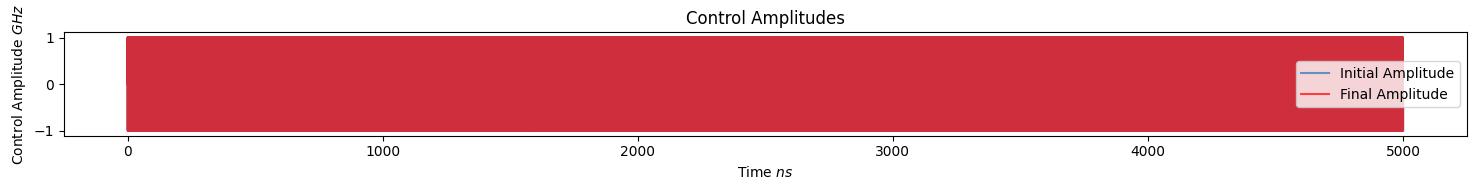
\includegraphics[width=0.95\linewidth]{vac2cat_effective_Hamiltonian_GRAPE_control1.png}
    \caption{vacuum to cat state control 1 pulse amplitudes}
    \label{fig:vac2cat_effective_Hamiltonian_GRAPE_control1}
\end{figure}
\begin{figure}[H]
    \centering
    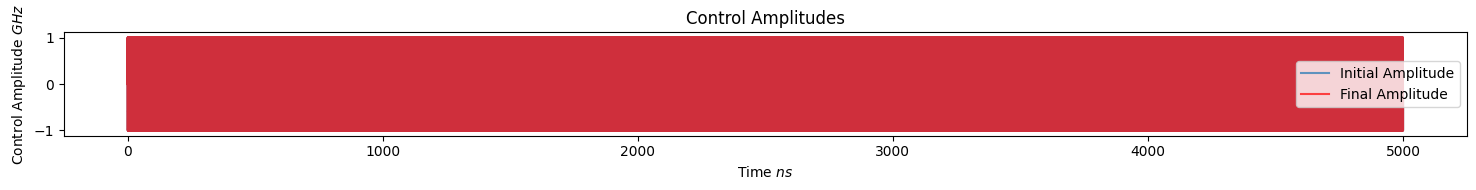
\includegraphics[width=0.95\linewidth]{vac2cat_effective_Hamiltonian_GRAPE_control2.png}
    \caption{vacuum to cat state control 2 pulse amplitudes}
    \label{fig:vac2cat_effective_Hamiltonian_GRAPE_control2}
\end{figure}
\begin{figure}[H]
    \centering
    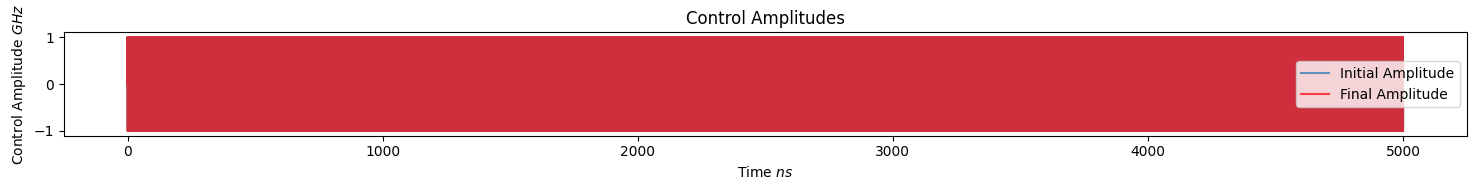
\includegraphics[width=0.95\linewidth]{vac2cat_effective_Hamiltonian_GRAPE_control3.png}
    \caption{vacuum to cat state control 3 pulse amplitudes}
    \label{fig:vac2cat_effective_Hamiltonian_GRAPE_control3}
\end{figure}

Forward simulation is given below to ensure that pulse optimization has run properly. 
\\
Simulation gives: 
\begin{itemize}
    \item sesolve final fidelity:  0.4390558062780975
    \item cavity ptrace fidelity:  0.44320315443027297
    \item qubit ptrace fidelity:  0.9871678390509413
    \item self-implemented final fidelity:  0.9529111010142354
\end{itemize}
\begin{figure}[H]
    \centering
    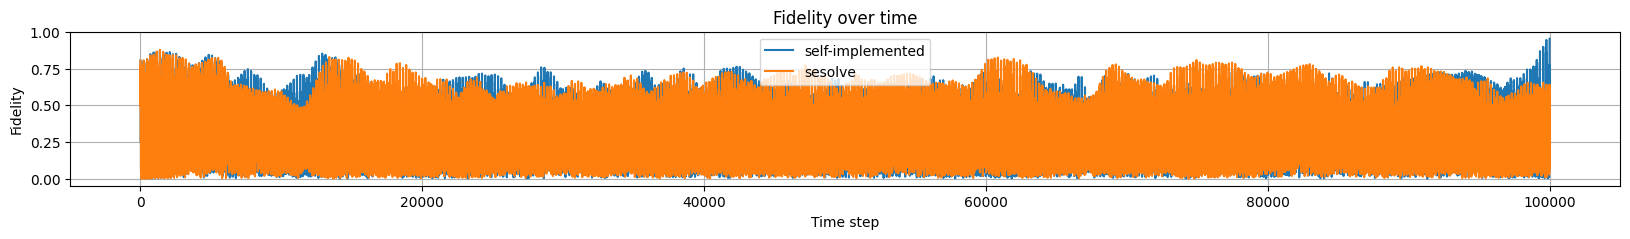
\includegraphics[width=0.95\linewidth]{vac2cat_effective_Hamiltonian_GRAPE_simulations.png}
    \caption{vacuum to cat state forward simulation}
    \label{fig:vac2cat_effective_Hamiltonian_GRAPE_simulations}
\end{figure}

It can be seen that the optimization results are not very satisfactory. 
Many tunings were attempted but none gave satisfactory results.
\\
At this point, we turned to look at a new python quantum control optimziation library, Krotov which builds on top of QuTip,
to see whether it can give better optimization results. Krotov’s optimization method is a gradient-based optimization algorithm like GRAPE. 
Krotov’s method distinguishes itself by guaranteeing monotonic convergence for near-continuous control fields. 
Besides the difference in optimization algorithm used, the Krotov package has the following incentives to be tried: 
\begin{itemize}
    \item Krotov is much better implemented than QuTip. For instance, Krotov allows display of optimization progress for every iteration. 
    \item Krotov allows inbuilds better customizability than QuTip. 
            For instance, Krotov allows for the optimization of the fidelity to be optimized.
\end{itemize}

Besides switching from QuTip to Krotov, the Hamiltonians are also redefined to be an interaction picture. 
The drift Hamiltonian ($H_0$) and control Hamiltonians ($H_1$, $H_2$, $H_3$) are defined as follows:

1. \textbf{Drift Hamiltonian} ($H_0$):
\begin{equation}
H_0 = \hbar \omega_r a^\dagger a + \frac{E_s}{2} \sigma_z + \frac{E_m}{2} \tau_z - \chi_m \tau_z \left(a^\dagger a + \frac{1}{2}\right) - \chi_s \sigma_z \left(a^\dagger a + \frac{1}{2}\right) - \frac{\chi_0}{2} \sigma_z \tau_z,
\end{equation}
where $\omega_r$ is the resonator frequency, $a$ and $a^\dagger$ are the annihilation and creation operators of the cavity, $E_s$ and $E_m$ are the energy levels of the qubit and the molecular orbital, $\sigma_z$ and $\tau_z$ are the Pauli Z operators for the qubit and the molecular orbital, respectively, and $\chi_m$, $\chi_s$, and $\chi_0$ are the dispersive shifts.

2. \textbf{Control Hamiltonians}:
   - $H_1$: This control Hamiltonian corresponds to the real part of the cavity drive. It is given by
     \begin{equation}
     H_1 = \left(a + a^\dagger\right),
     \end{equation}
     where $a$ and $a^\dagger$ are the annihilation and creation operators of the cavity.

   - $H_2$: This control Hamiltonian corresponds to the imaginary part of the cavity drive. It is given by
     \begin{equation}
     H_2 = -i\left(a - a^\dagger\right),
     \end{equation}
     where $a$ and $a^\dagger$ are the annihilation and creation operators of the cavity.

   - $H_3$: This control Hamiltonian corresponds to the drive on the qubit. It is given by
     \begin{equation}
     H_3 = \sigma_x,
     \end{equation}
     where $\sigma_x$ is the Pauli X operator for the qubit.
\\
The optimized results are as follow. 
\begin{figure}[H]
    \centering
    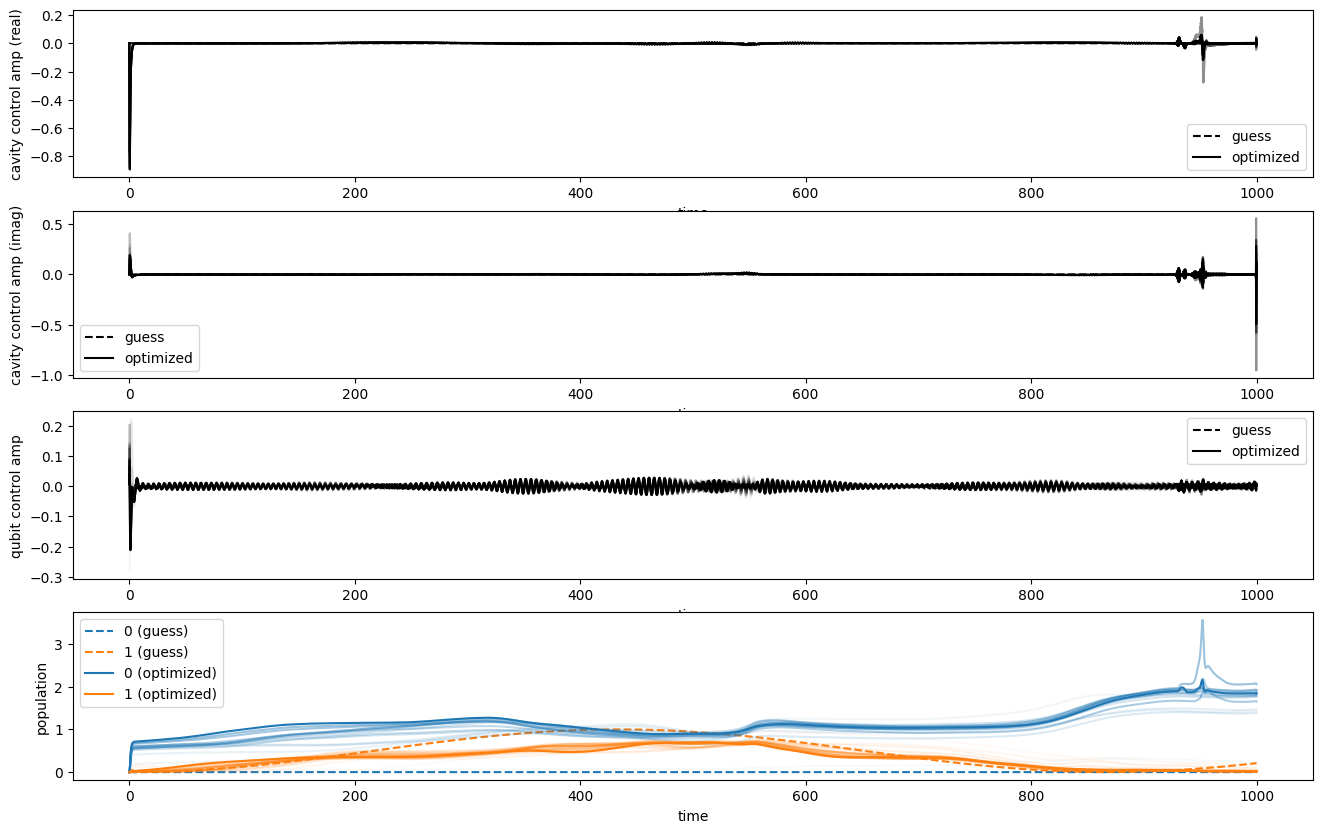
\includegraphics[width=0.95\linewidth]{vac2cat_krotov.png}
    \caption{
        (1st,2nd) The optimized control fields for the cavity drive (real and imaginary parts) and the qubit drive. \\
        (3rd) qubit control \\
        (4th) qubit population
    }
    \label{fig:vac2cat_krotov}
\end{figure}

Forward simulation is given below to ensure that pulse optimization has run properly. 
\\
Simulation gives: 
\begin{itemize}
    \item final fidelity:  0.9992259750482354
\end{itemize}

\begin{figure}[H]
    \centering
    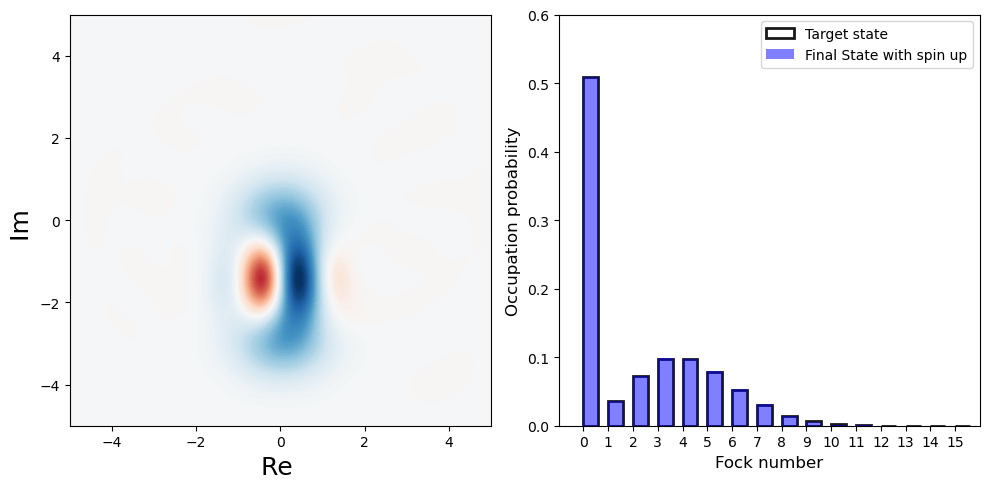
\includegraphics[width=0.95\linewidth]{vac2cat_simulation.png}
    \caption{
       (left) Wigner function representation of target cavity state and final cavity state 
       \\
       (right) target cavity state and final cavity state in Fock state basis
    }
    \label{fig:vac2cat_simulation}
\end{figure}



%%%%%%%%%%%%%%%%%%%%%%%%%%%%%%%
\subsection{Further discussions reagarding numerical pulse optimzation}
\begin{enumerate}
    \item choosing time parameters: 
        \begin{itemize}
            \item evolution time (evo\_time): pulse length needed can be estimated %TODO: ask chiyuan how is this calculated
            \item number of time slices (n\_ts): n\_ts that is too small will lead to large error; 
                n\_ts that is too large will result in long computation time; 
                hence an appropriate n\_ts value needs to be tested via trial and error.
        \end{itemize}
\end{enumerate}

%%%%%%%%%%%%%%%%%%%%%%%%%%%%%%%%%%%%%%%%%%%%%%%%%%%%%%%%%%%%%%%
\section{Future work}\label{sec:future_work}
\begin{itemize}
    \item Try the last code in rotating frame to alleviate fast oscillations in optimized pulses
    \item fudelity partial trace over cavity state
    \item compare with fidelity when using original full Hamiltonian 
    \item gate design 
    \item consdier noise
\end{itemize}

\section{Conclusion}
To be filled.

\appendix
\section{EXACT DIAGONALIZATION OF THE DOUBLE-QUANTUM-DOT HAMILTONIAN}
The DQD Hamiltonian, Eq. \ref{eq:DQD_Hamiltonian}, may be diagonalized exactly in three steps. 
First, we write Eq. \ref{eq:DQD_Hamiltonian} in the eigenbasis of the molecular Hamiltonian. This is done with the transformation
$$
U_0=\exp \left[-i \frac{(\pi / 2-\theta)}{2} \widetilde{\tau}_y\right]
$$
The transformed Hamiltonian takes the form
$$
\begin{aligned}
U_0^{\dagger} H_d U_0= & \frac{\Omega}{2} \widetilde{\tau}_z+\frac{B_z}{2} \widetilde{\sigma}_z+\frac{b_x \sin \theta}{2} \widetilde{\tau}_z \widetilde{\sigma}_x \\
& -\frac{b_x \cos \theta}{2} \widetilde{\tau}_x \widetilde{\sigma}_x .
\end{aligned}
$$

Second, the spin basis is rotated to match the direction of the total magnetic field $\mathbf{B}=\left(b_x \sin \theta, 0, B_z\right)$. This is achieved through the unitary transformation
\begin{equation}
    U_1=\exp \left(-i \frac{\Phi}{2} \widetilde{\tau}_z \widetilde{\sigma}_y\right) .    
\end{equation}


Here $\Phi$ is the angle between the magnetic field and the $z$ axis, satisfying $\tan \Phi=b_x \sin \theta / B_z$. In the doubly transformed basis, the DQD Hamiltonian takes the form
\begin{equation}\label{eq:A4}
    \begin{aligned}
        & U_1^{\dagger} U_0^{\dagger} H_d U_0 U_1 \\
        & \quad=\frac{\Omega}{2} \widetilde{\tau}_z+\frac{B_z \sec \Phi}{2} \widetilde{\sigma}_z-\frac{b_x \cos \theta}{2} \widetilde{\tau}_x \widetilde{\sigma}_x .
    \end{aligned}
\end{equation}

The Hamiltonian of Eq. \ref{eq:A4} preserves the parity quantum number $\tilde{\tau}_z \tilde{\sigma}_z$. Thus, it may be diagonalized separately for each parity. The corresponding unitary transformation is
$$
\begin{aligned}
& U_2=U_{2+}+U_{2-}, \\
& U_{2+}=\cos \frac{\phi_{+}}{2} P_{+}-\sin \frac{\phi_{+}}{2}\left(\tilde{\tau}_{-} \tilde{\sigma}_{-}-\tilde{\tau}_{+} \tilde{\sigma}_{+}\right), \\
& U_{2-}=\cos \frac{\phi_{-}}{2} P_{-}-\sin \frac{\phi_{-}}{2}\left(\tilde{\tau}_{-} \tilde{\sigma}_{+}-\tilde{\tau}_{+} \tilde{\sigma}_{-}\right),
\end{aligned}
$$
where $P_{ \pm}=\left(1 \pm \tilde{\tau}_z \widetilde{\sigma}_z\right) / 2$ are the projectors on the subspaces of parity $\pm$, respectively. The effective spin-orbit mixing angles are determined by
$$
\tan \phi_{ \pm}=\frac{b_x \cos \theta}{\Omega \pm B_z \sec \Phi} .
$$

Defining the total unitary transformation $U=U_0 U_1 U_2$, the DQD Hamiltonian becomes
\begin{equation}\label{eq:A7}
    U^{\dagger} H_d U=\frac{E_m}{2} \widetilde{\tau}_z+\frac{E_s}{2} \widetilde{\sigma}_z,
\end{equation}

where the molecular and spin Larmour frequencies in the dressed basis are
\begin{equation}\label{eq:A8}
    \begin{aligned}
        E_m & =\frac{b_x \cos \theta}{2}\left(\csc \phi_{+}+\csc \phi_{-}\right), \\
        E_s & =\frac{b_x \cos \theta}{2}\left(\csc \phi_{+}-\csc \phi_{-}\right) .
        \end{aligned}
\end{equation}

To indicate the final DQD eigenbasis, the explicit unitary transformation as well as the " ," are dropped. Equation \ref{eq:A7} then becomes Equation \ref{eq:DQD_Hamiltonian_in_eigenbasis}.

The resonator couples to the $\underset{\sim}{\mathrm{DQD}}$ via the dimensionless position operator $\zeta=|\widetilde{R}\rangle\langle\widetilde{R}|-| \widetilde{L}\rangle\langle\widetilde{L}|$. 
The unitary transformation of Eq. \ref{eq:A7} may be used to express $\zeta$ in the DQD eigenbasis as
$$
\zeta=\sum_{i, j} \zeta^{(i j)} \tau_i \sigma_j
$$

Here the Pauli matrices are labeled with indices $\{0, x, y, z\}$, where 0 signifies the identity matrix. The nonzero coefficients
$\zeta^{(i j)}$ are found to be
\begin{equation}\label{eq:A10}
    \begin{aligned}
        \zeta^{(x 0)}= & -\cos \theta \cos \Phi \cos \bar{\phi}, \\
        \zeta^{(z x)}= & \cos \theta \cos \Phi \sin \bar{\phi}, \\
        \zeta^{(x x)}= & \sin \theta \sin \bar{\phi} \cos \frac{\Delta \phi}{2} \\
        & +\cos \theta \sin \Phi \sin \bar{\phi} \sin \frac{\Delta \phi}{2}, \\
        \zeta^{(y y)}= & -\sin \theta \cos \bar{\phi} \sin \frac{\Delta \phi}{2} \\
        & +\cos \theta \sin \Phi \cos \bar{\phi} \cos \frac{\Delta \phi}{2}, \\
        \zeta^{(z 0)}= & \sin \theta \cos \bar{\phi} \cos \frac{\Delta \phi}{2} \\
        & +\cos \theta \sin \Phi \cos \bar{\phi} \sin \frac{\Delta \phi}{2}, \\
        \zeta^{(0 z)}= & -\sin \theta \sin \bar{\phi} \sin \frac{\Delta \phi}{2} \\
        & +\cos \theta \sin \Phi \sin \bar{\phi} \cos \frac{\Delta \phi}{2} .
        \end{aligned}
\end{equation}


In Eq. \ref{eq:A10}, we have introduced the average spin-orbit mixing angle $\bar{\phi}=\left(\phi_{+}+\phi_{-}\right) / 2$ and the difference angle $\Delta \phi=$ $\phi_{+}-\phi_{-}$. 
Expressions for the DQD-resonator couplings appearing in Eq. \ref{eq:DQD_resonator_interaction_new_basis} are directly obtained from the $\zeta^{(i j)}$ :
\begin{equation}\label{eq:A11}
    \begin{aligned}
        g_m & =-g_c \zeta^{(x 0)}, & & g_s=g_c \zeta^{(z x)}, \\
        g_{+} & =g_c\left[\zeta^{(x x)}-\zeta^{(y y)}\right], & g_{-} & =g_c\left[\zeta^{(x x)}+\zeta^{(y y)}\right], \\
        g_{m p} & =g_c \zeta^{(z 0)}, & & g_{s p}=g_c \zeta^{(0 z)} .
        \end{aligned}
\end{equation}
In the limit of small field gradient discussed in Sec. II B, Eqs. \ref{eq:A8} and \ref{eq:A11} yield Eqs. \ref{eq:Larmour_frequencies} and \ref{eq:couplings}, respectively. 
Moreover, note that the matrix element of the dimensionless position operator $\zeta$ between the two spin-qubit states is proportional to $g_s / g_c$. 
This means that spin transitions arising from the coupling of electric fields to the electric dipole occur at a rate proportional to $\left(g_s / g_c\right)^2$. 
Finally, we remark that exact expressions for the transformed spin operators may also be obtained.

\printbibliography
\end{document}